\documentclass[titlepage,11pt]{article}

\textwidth 6.5in
\textheight 9in
\oddsidemargin -0.2in
\topmargin -0.5in

\usepackage{indentfirst,graphics,alltt,epsfig,color}

\title{iBioSim User's Manual}

\author{Chris J. Myers, Nathan Barker, Kevin Jones, Hiroyuki Kuwahara,\\ Curtis
  Madsen, Nam Nguyen, Tyler Patterson, Nicholas Roehner, Jason Stevens} 

% \date{Created: August 6th, 2008\\
%   Last Revised: October 2, 2010
% }

\begin{document}

\maketitle

%show only subsection granularity in the toc
%\setcounter{tocdepth}{2} 
  
\tableofcontents

\clearpage
  
%\setlength{\parindent}{0em}
%\setlength{\parskip}{10pt}

\section{Introduction}

\noindent
{\tt iBioSim} has been developed for the modeling, analysis, and design of genetic circuits.  While {\tt iBioSim} primarily targets models of genetic circuits, models representing metabolic networks, cell-signaling pathways, and other biological and chemical systems can also be analyzed.  Recently, modeling and visualization support has been added for static multi-cellular and spatial models as well.
It is capable of importing and exporting models specified using the %%tth:\begin{html}<A HREF="http://www.sbml.org/">\end{html}
\emph{Systems Biology Markup Language}
%%tth:\begin{html}</A>\end{html}
~(SBML).  It can import all levels and versions while being able to export Level 2 Version 4 or Level 3 Version 1.  It supports all SBML modeling constructs except the \emph{delay} function and some types of \emph{fast} reactions.  It was the first tool to produce correct results for all examples in the SBML benchmark suite.  It has also been tested successfully on the stochastic benchmark suite and the curated models in the 
%%tth:\begin{html}<A HREF="http://www.ebi.ac.uk/biomodels-main/">\end{html}
\emph{BioModels database}.
%%tth:\begin{html}</A>\end{html}
Finally, it is one of the first tools to also support the 
%%tth:\begin{html}<A HREF="http://www.sbolstandard.org/">\end{html}
\emph{Synthetic Biology Open Language}
%%tth:\begin{html}</A>\end{html}  
(SBOL), an emerging standard for information exchange in synthetic biology.
{\tt iBioSim} includes the following components: 
\begin{itemize}
\item Model Editor - a tool to create a model of a genetic circuit or other biological system.
%% TODO: FIX THIS
%\item LPN Model Editor - a tool to create a model using a \emph{labeled Petri net} (LPN).
\item SBOL Browser - a tool to view SBOL files and associate DNA components to model elements.
\item Analysis Tool - an abstraction-based ODE, Monte Carlo, and Markov analysis tool.
\item Learn Tool - a tool to learn a model from \emph{time series data} (TSD).
\item TSD Graph Editor- a tool to visualize TSD files. 
\item Histogram Graph Editor - a tool to visualize probability data. 
\end{itemize}

\section*{Credits}

\noindent
The iBioSim tool is being developed at the University of Utah
by 
%%tth:\begin{html}<A HREF="http://www.async.ece.utah.edu/~myers">\end{html}
Chris Myers, 
%%tth:\begin{html}</A>\end{html}
%%tth:\begin{html}<A HREF="http://www.cs.utah.edu/~barkern">\end{html}
Nathan Barker, 
%%tth:\begin{html}</A>\end{html}
%%tth:\begin{html}<A HREF="http://www.async.ece.utah.edu/~kjones">\end{html}
Kevin Jones, 
%%tth:\begin{html}</A>\end{html}
%%tth:\begin{html}<A HREF="http://www.cs.utah.edu/~kuwahara">\end{html}
Hiroyuki Kuwahara, 
%%tth:\begin{html}</A>\end{html}
%%tth:\begin{html}<A HREF="http://www.async.ece.utah.edu/~cmadsen">\end{html}
Curtis Madsen, 
%%tth:\begin{html}</A>\end{html}
%%tth:\begin{html}<A HREF="http://www.cs.utah.edu/~namphuon">\end{html}
Nam Nguyen, 
%%tth:\begin{html}</A>\end{html}
%%tth:\begin{html}<A HREF="http://www.cs.utah.edu/~patterson">\end{html}
Tyler Patterson, 
%%tth:\begin{html}</A>\end{html}
Nicholas Roehner, 
and Jason Stevens.  Nathan Barker is now with Southern Utah University, Kevin Jones is now with Raytheon, Hiroyuki Kuwahara is now with Carnegie Mellon University, and Nam Nguyen is now with the University of Texas in Austin.

\clearpage

\section{Project Management}

\noindent
Within {\tt iBioSim}, all files are collected within projects.   
A project is a collection of models, analysis views, learn views, and graphs.  As shown below, {\tt iBioSim} displays all project files on the left; the open models, views, and graphs on the right; and a log of all external commands on the bottom.  The menu bar is located on the top of the window in the Windows and Linux versions.  It is located on the top of the screen in the MacOS version.

\begin{center}

\includegraphics[height=90mm]{screenshots/iBioSim}
\end{center}

\clearpage

\subsection{Creating and Opening Projects}

\noindent
To create a new project, select New $\rightarrow$ Project from the File menu as shown below.  You will then be prompted to browse to a desired location and to give a name to the project directory.  After you do this, click the new button and a new project directory will be created.  To open a project, select Open $\rightarrow$ Project from the File menu.  You will then be prompted to browse to a project directory to open, and clicking open will open the project. You may also open a project by selecting one of your ten most recently opened projects by selecting the project name shown in the File drop down menu shown below. 

\begin{center}
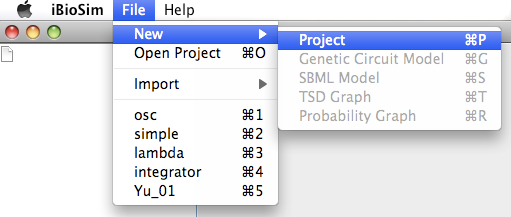
\includegraphics[height=80mm]{screenshots/project}
\end{center}

\clearpage

\subsection{Creating and Opening Models and Graphs}

\noindent
After you have created or opened a project, you can create a new model or graph to add to the project.  To create a new model, select New $\rightarrow$ Model from the File menu as shown below. You will then be prompted to enter a model ID.  At this point, a Model editor (see Section~\ref{ModelEdit}) will open in a new tab.  To create a new LPN model, select New $\rightarrow$ LPN Model from the File menu. You will then be prompted to give a model ID.  At this point, an LPN model editor 
%% TODO:
%(see Section~\ref{LPNEdit}) 
will open in a new tab. To create a new TSD graph, select New $\rightarrow$ TSD Graph from the File menu. You will then be prompted to give a name to the TSD graph.  At this point, a TSD graph editor (see Section~\ref{TSDGraph}) will open in a new tab. To create a new histogram, select New $\rightarrow$ Histogram from the File menu. You will then be prompted to give a name to the histogram.  At this point, a histogram editor (see Section~\ref{Histogram}) will open in a new tab.  Once a model or graph is created, it can be opened again later by right-clicking on the object in the project window and selecting ``View/Edit'' or, alternatively, double-clicking on the object.  Note that a model can be opened in either a graphical or textual editor.  An open model or graph can be closed by either clicking on the ``X'' in the tab or by selecting File $\rightarrow$ Close.  The File $\rightarrow$ Close All option will close all tabs.

\begin{center}
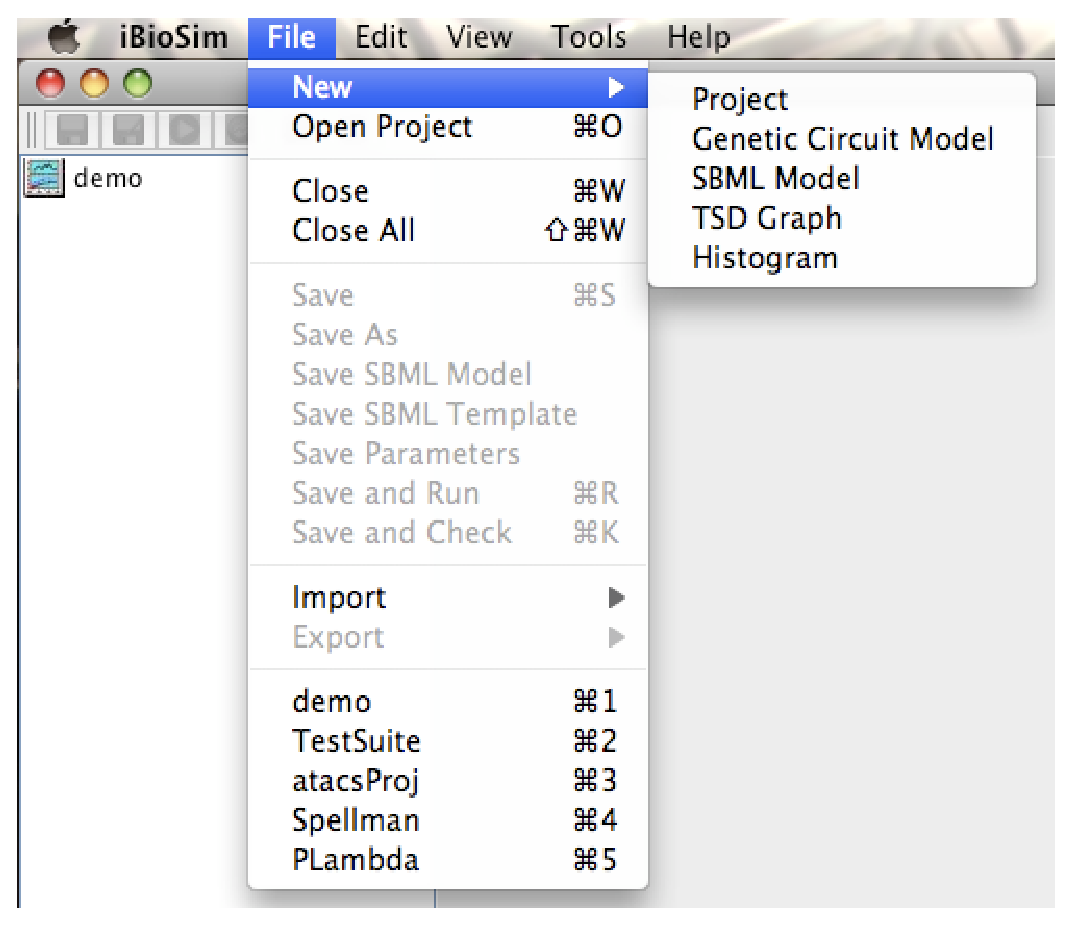
\includegraphics[height=80mm]{screenshots/newModel}
\end{center}

\clearpage

\subsection{Importing Models}

\noindent
You can also import models into the current working project.  These can be models from other {\tt iBioSim} projects, models in the 
%%tth:\begin{html}<A HREF="http://www.sbml.org/">\end{html}
\emph{Systems Biology Markup Language}
%%tth:\begin{html}</A>\end{html}
~(SBML), models from the
%%tth:\begin{html}<A HREF="http://www.ebi.ac.uk/biomodels-main/">\end{html}
\emph{BioModels database}
%%tth:\begin{html}</A>\end{html}
, LPN models, or a 
%%tth:\begin{html}<A HREF="http://www.sbolstandard.org/">\end{html}
\emph{Synthetic Biology Open Language}
%%tth:\begin{html}</A>\end{html}  
(SBOL) file (see Section~\ref{SBOL}). 
To import an {\tt iBioSim} model, select File $\rightarrow$ Import $\rightarrow$ iBioSim Model.  
You will then be able to browse to find a model to import.  After  selecting the desired model, click the import button to bring the model into the project.  Before bringing the model into the project, it will be checked to see if it is a valid model file.  To import an SBML model, the procedure is the same except use the Import $\rightarrow$ SBML Model option.  Before bringing the model into the project, it will be checked to see if it a valid SBML file.  
The model will also be checked for consistency, and any errors or warnings will be reported.  These should be corrected before analysis of the model is performed.  Importing of an LPN model or an SBOL file are similar in that you are asked to locate the appropriate file to import.

\begin{center}
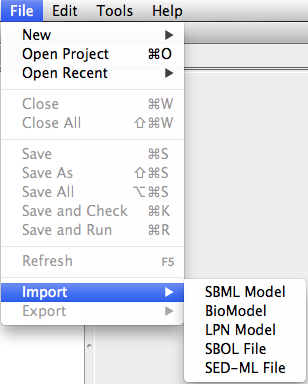
\includegraphics[height=80mm]{screenshots/import}
\end{center} 

When importing a model from the BioModels database, the window below will open, initially only listing the BioModel numbers.  Selecting ``Get Names'' will fetch the model names from the database.  Beware that this can take a significant amount of time.  When you click on a model to select it, you can use the ``Get Description'' button to fetch a description of the model which will open in a browser.  Similarly, the ``Get Reference'' button will fetch the reference describing this model and again open it in a browser.

\begin{center}
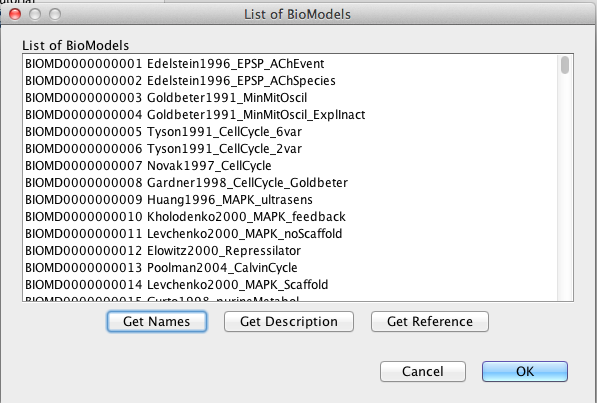
\includegraphics[height=80mm]{screenshots/BioModels}
\end{center} 

\subsection{Exporting Models and Graphs}

\noindent
You can also export a model in either SBML or SBOL format.  To export an SBML model, select File $\rightarrow$ Export $\rightarrow$ Systems Biology Markup Language (SBML).  Then, you will be able to browse to find a location to export the SBML file.  Currently, the SBML model generated is a single flattened chemical reaction model.  When exporting model as an SBOL component, you must browse to find an SBOL library.  The SBOL component will then be added to the selected library.  Graphs of time series data or histograms can be exported from the project in many formats.  The supported file formats are:  
\begin{itemize}
\item Time series data format (tsd), see Section~\ref{TSD}..
\item Comma separated value (csv).
\item Column separated data (dat).
\item Encapsulated postscript (eps). 
\item Joint Photographic Experts Group (jpg). 
\item Portable document format (pdf).
\item Portable network graphics (png). 
\item Scalable vector graphics (svg).
\end{itemize}

\clearpage

\subsection{Editing Project Objects and Creating Tool Views}

\noindent
All project objects can be modified by highlighting the object and using a right mouse click to open a menu of options, as shown below. Using this menu, every type of object can be copied, renamed, or deleted (these actions can also be done from the Edit menu).  For a model file, the ``View/Edit'' option opens the model editor (see Section~\ref{ModelEdit}).  For an LPN model, the ``View/Edit'' option opens the LPN model editor. 
% TODO:
% (see Section~\ref{LPNEdit}).
For a TSD graph, the ``View/Edit'' option opens the TSD graph editor (see Section~\ref{TSDGraph}).  For a histogram, the ``View/Edit'' option opens the histogram graph editor 
(see Section~\ref{Histogram}).  
% For an analysis view, the ``Open Analysis View'' option opens the analysis view (see Section~\ref{Analysis}). For a learn view, the ``Open Learn View'' option opens the learn view (see Section~\ref{Learn}).

\begin{center}
%\begin{tabular}{ccc}
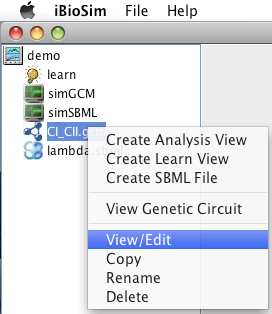
\includegraphics[height=65mm]{screenshots/modGCM} 
%& &
%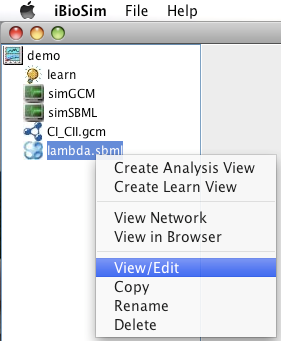
\includegraphics[height=65mm]{screenshots/modSBML} \\ \\
%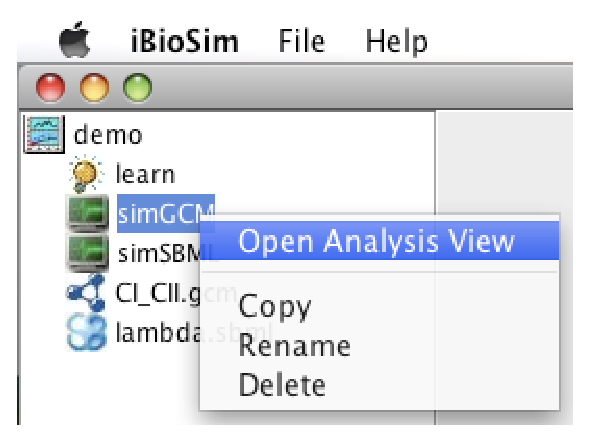
\includegraphics[height=35mm]{screenshots/modAnalysis} & &
%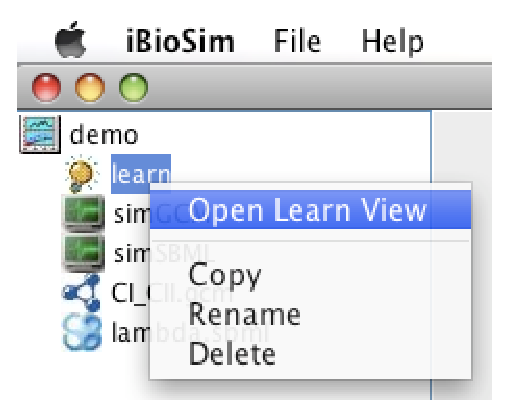
\includegraphics[height=35mm]{screenshots/modLearn}
%\end{tabular}
\end{center}

% \subsection{Viewing Project Objects}

% \noindent
% A GCM can also be viewed using 
% %%tth:\begin{html}<A HREF="http://www.graphviz.org/">\end{html}
% GraphViz's
% %%tth:\begin{html}</A>\end{html}
% dotty program  by right clicking on the model you want to view and              
% selecting the ``View Genetic Circuit'' option. 
% There are two additional ways to view an SBML model. You
% can either select the ``View Network'' option or the
% ``View in Browser'' option.  The ``View Network''
% option converts the model to a GraphViz file and then will open that 
% file with GraphViz's dotty program.  The ``View in Browser'' option 
% coverts the model to an xhtml file and opens that file with your 
% default xhtml browser.  These options can also be reached using the
% View $\rightarrow$ Model sub-menu.
% \begin{center}
% \begin{tabular}{ccc}
% 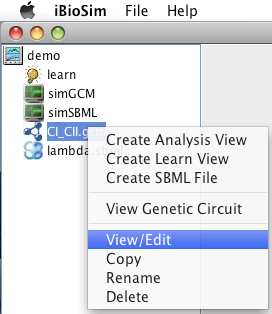
\includegraphics[height=65mm]{screenshots/modGCM} & &
% 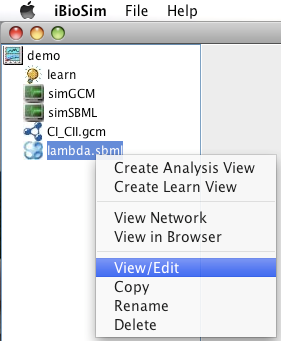
\includegraphics[height=65mm]{screenshots/modSBML} \\ \\
% 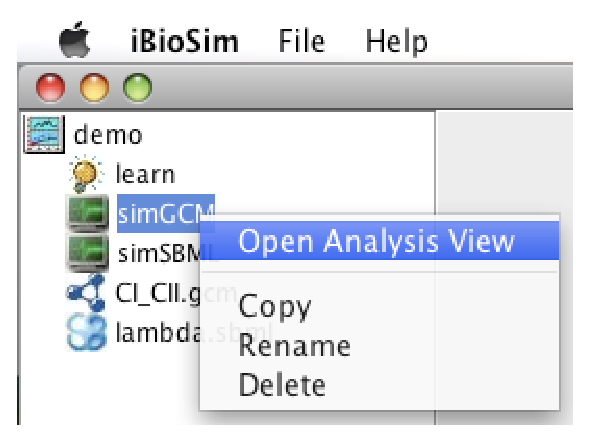
\includegraphics[height=35mm]{screenshots/modAnalysis} & &
% 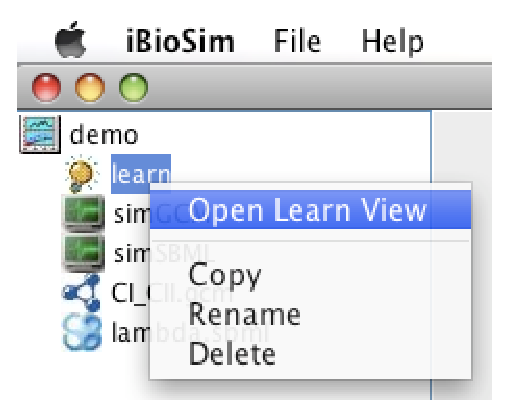
\includegraphics[height=35mm]{screenshots/modLearn}
% \end{tabular}
% \end{center}

% \clearpage

% \subsection{Creating Tool Views}

\noindent
To perform analysis or learning, right-click on a model and select ``Create Analysis View'' (see Section~\ref{Analysis}) to perform analysis or ``Create Learn View'' (see Section~\ref{Learn}) to perform learning. You will then be prompted to give a name to your analysis or learn view. After a name is entered, a tab with the newly created view will open.  Views can also be created using the Tools menu.  Once a view is created, it can be opened again later by right-clicking on an analysis directory and selecting ``Open Analysis/Learn View'' or, alternatively, double-clicking on the view.

% \begin{center}
% \begin{tabular}{ccc}
% 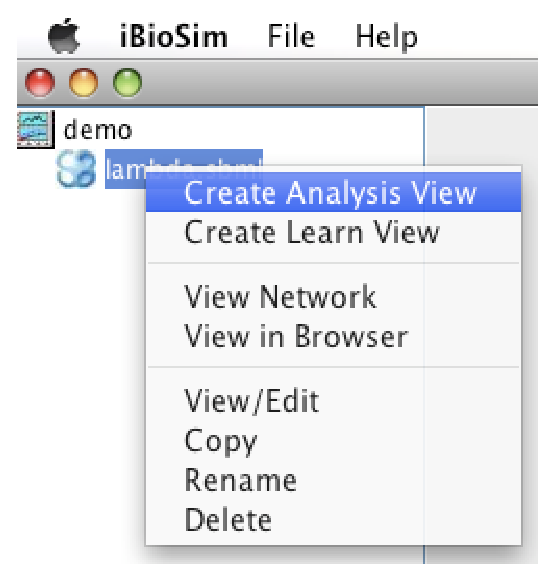
\includegraphics[height=55mm]{screenshots/createAnalysis} & & 
% 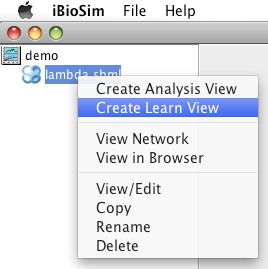
\includegraphics[height=55mm]{screenshots/createLearn}
% \end{tabular}
% \end{center}

\clearpage

\section{\label{ModelEdit}Model Editor}

\noindent
The model editor allows the user to create or modify a model of a genetic circuit or other biochemical system.  {\tt iBioSim} models are based on SBML Level 3 Version 1 models with added features to support visualization, hierarchy, and modeling of genetic regulation.  SBML models can be imported and exported to allow interfacing with SBML-compliant tools.  When exporting an SBML model, the hierarchy and genetic regulation are flattened to create a single SBML model.  The model editor includes both a schematic editor as well as several textual editors.  For large models, the schematic portion can also be edited textually instead.  As shown below, when creating a new model, you can select whether the model should be on a grid or not.  Let us focus initially on models that are not on a grid.

\begin{center}
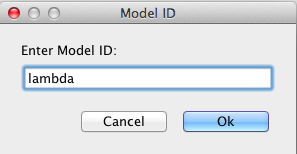
\includegraphics[height=25mm]{screenshots/ModelId}
\end{center}

\noindent
The schematic editor shown below allows one to add \emph{chemical species} (see Section~\ref{Species}), 
\emph{chemical reactions} (see Section~\ref{Reactions}), \emph{components} (see Section~\ref{Components}),
and \emph{promoters} (see Section~\ref{Promoters}) to a model depending on the icon selected in the toolbar.   Chemical species are the molecules such as proteins.  Chemical reactions change \emph{reactant} species into \emph{product} species.  Components are instances of other models within the project.  Finally, promoters are locations on a DNA sequence in which transcription is initiated.  
% 
There are several types of relationships between species that can be specified.  A species may \emph{activate} or \emph{repress} the production of other species (see Section~\ref{Influences}).  One can also specify when there is no influence between two species or when a self-influence exists.  Species can also be related by complex-formation reactions  which indicate that multiple identical or different species can be combined to form a complex species.  A species can also be a reactant or product in a chemical reaction, indicating that the reaction consumes or produces the species, respectively (see Section~\ref{Reactions}).  Finally, a species can be a \emph{modifier} to a chemical reaction, indicating that it affects the rate of the reaction but is neither produced nor consumed by the reaction (see Section~\ref{Reactions}).
%
The next item on the toolbar is a checkbox used to indicate if the model is to be considered enclosed within a \emph{compartment}.  The combo box is used to select the enclosing compartment for the model.  The remaining items on the toolbar allow you to apply an automatic layout routine 
\includegraphics{../gui/icons/modelview/choose_layout_selected}, zoom, restore to default size (Un-Zoom), pan, undo, and redo.
% 
Finally, the additional tabs allow the user to add, edit, or remove compartments (membrane-enclosed objects where reactions take place, see Section~\ref{Compartments}), \emph{parameters} (values used in model generation and within math equations, see Section~\ref{Parameters}), \emph{definitions} (custom functions and units, see Section~\ref{Definitions}), \emph{assignments} (mathematical equations that govern the values of variables in the model, see Section~\ref{Assignments}), \emph{properties} (mathematical equations that describe either desired or undesired behaviors, see Section~\ref{Properties}), and \emph{events} (objects that describe discrete state changes, see Section~\ref{Events}).

\begin{center}
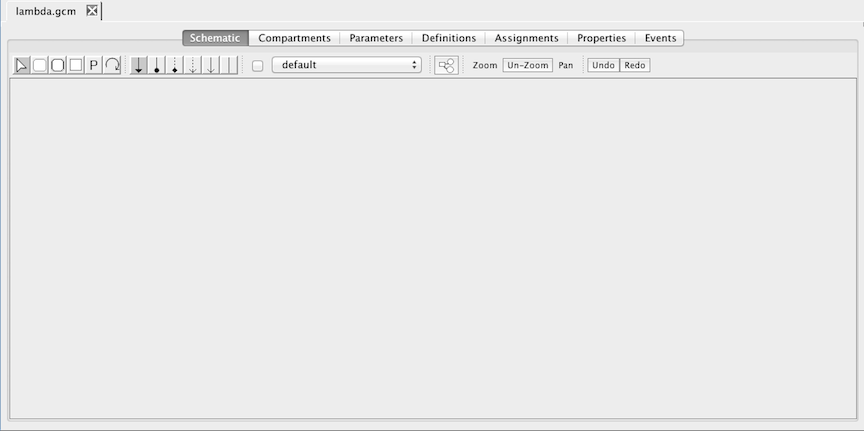
\includegraphics[height=80mm]{screenshots/ModelEditor}
\end{center}

\noindent
{\tt iBioSim} also supports the creation of models on a grid.  The idea of a grid is to provide a coarse-grain spatial representation.  A single model can be instantiated within each grid location.  The models can be for individual cells, allowing one to model population dynamics.  The models can also be different segments of a single cell, allowing one to model diffusion within a cell.  Key to grid-based modeling are diffusible species, described in Section~\ref{Species}.  When the models within grid locations are compartment-enclosed components, reactions are added to represent the movement of these diffusible species between the compartment and the area outside the compartment within the grid location (i.e., membrane diffusion).  When performing analysis, reactions are also automatically added to represent the movement of these diffusible species between the grid locations.  To use a grid, check the Make Grid option when creating the model.  A window will then open asking for the number of rows and columns in the grid.  It also asks which model to use to populate the grid.  You can select ``none'' if you wish to populate it later.

\begin{center}
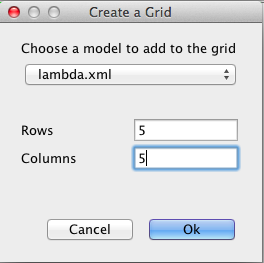
\includegraphics[height=40mm]{screenshots/createGrid}
\end{center}

The schematic for a model on a grid is a bit different than for an ordinary model, which is evident from the toolbar.  Namely, a grid-based model can only include components, with at most one component per grid location.  By pressing the Add Component icon 
\includegraphics{../gui/icons/modelview/add_component_selected} and clicking on an empty grid location, you are allowed to select a model to instantiate within that grid location.  You can also select Edit Grid Size to change the size of the grid.  If the grid is larger in one or more dimensions than before, you can select a model to populate the new grid locations.  A smaller grid size simply removes the component instantiations that fall outside the new grid.  You can also edit the grid by selecting individual grid locations by clicking on them or selecting multiple grid locations using the rectangle selection tool by left-clicking and dragging the mouse.  When you then use the right mouse button, it brings up the menu shown below.  This menu allows you to delete the component that was right-clicked on or to open its model in a Model Editor.  You can also use this menu to select or de-select all grid locations, and you can either clear occupied, or populate non-occupied, selected grid locations.

\begin{center}
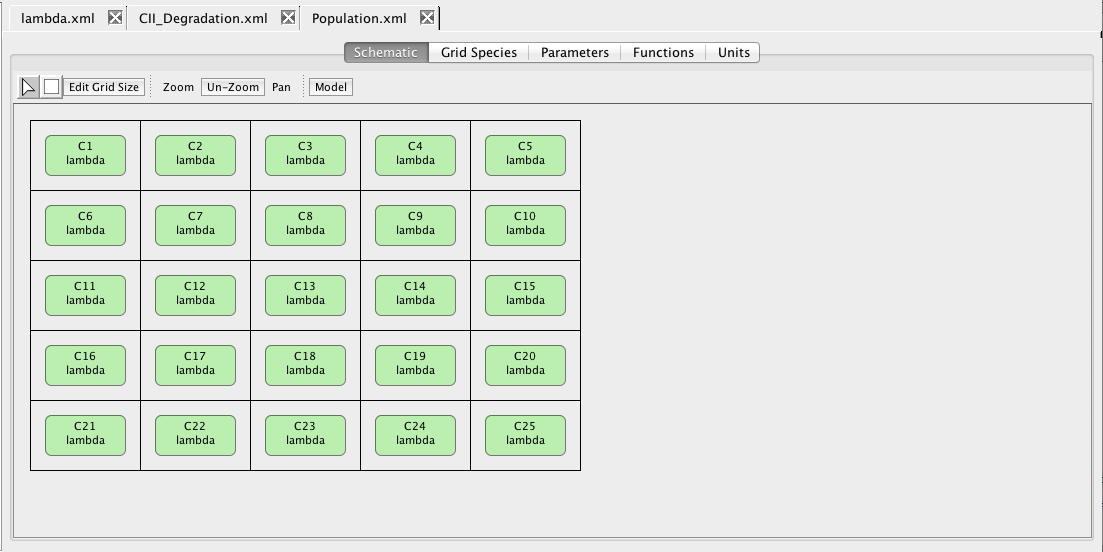
\includegraphics[height=80mm]{screenshots/gridModel}
\end{center}

\begin{center}
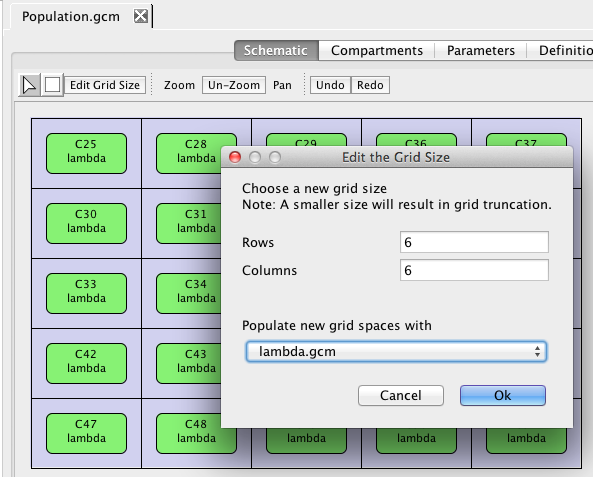
\includegraphics[height=80mm]{screenshots/editGridSize}
\end{center}

\begin{center}
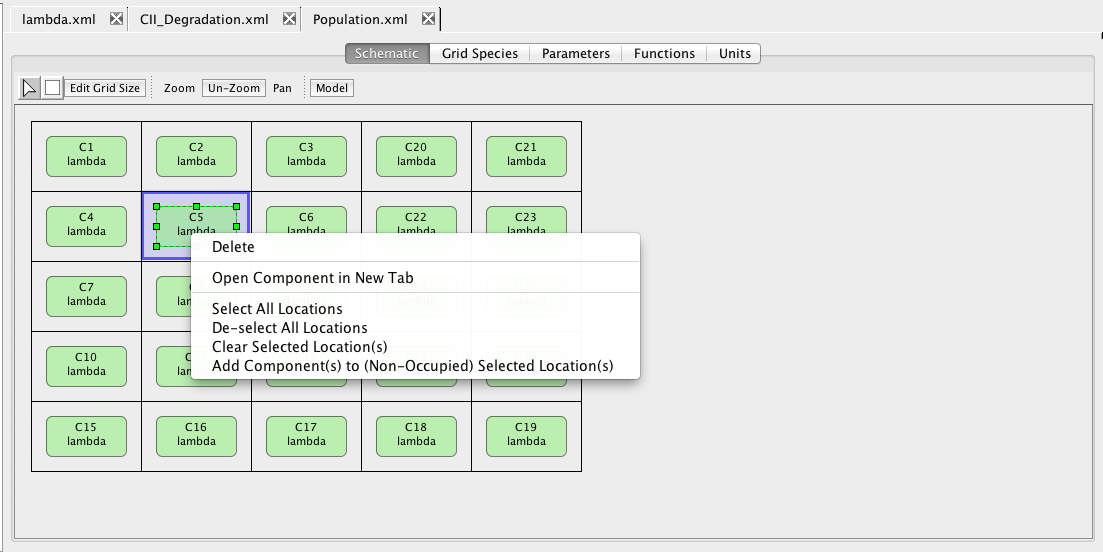
\includegraphics[height=80mm]{screenshots/gridRightButton}
\end{center}

\subsection{\label{Species}Species}

\noindent
Species are the molecules, such as proteins, that are produced by genes or chemical reactions.  To add a species to the model, select the Add Species icon 
\includegraphics{../gui/icons/modelview/add_species_selected} and click on the schematic canvas.  This will drop a new species with default ID and other values.  You may change these defaults by double-clicking on the species to open the Species Editor.  A species has the following elements:
\begin{itemize} 
\item ID: a unique ID composed of only alphanumeric characters and underscores.
\item Name: an arbitrary string description of the species (optional).
\item Type: used to indicate how this species can be connected in hierarchical models.  The \emph{input} type is used to indicate a species that is produced outside this model, the \emph{internal} type is used to indicate that a species is produced inside this model but cannot be used in other models, and the \emph{output} type is used to indicate that a species is produced by this model and can be used in other models. 
\item Diffusible: this checkbox indicates if this species can diffuse in multi-compartment and grid-based models.
\item Constitutive: this checkbox indicates that a default production reaction should be created for this species.
\item Compartment: location of the species (default=default).
\item Boundary Condition: Boolean indicating if the species amount/concentration cannot be changed by reactions (default=false).
\item Constant: Boolean indicating if the species amount/concentration is constant (default=false).
\item Has Only Substance Units: Boolean indicating if the species is to be considered an amount in mathematical equations (default=true).
\item Units: the units for the amount/concentration (default=none).
\item Conversion Factor: is a constant global parameter, the value of which is used to convert this species' units into the units used for extent (i.e., the units of change due to reactions).
\item Initial amount/concentration (ns): initial value of the amount or concentration of the species.  If the value is enclosed in brakets (i.e., $[number]$), it is a concentration, otherwise it is an amount.  The default is the value of the global parameter ns.
\item Degradation rate (kd): the degradation rate for this species.  The default is the value of the global parameter kd.  Note that a value of 0 will result in no degradation reaction being produced for this species.
\item Extracellular degradation rate (kecd): the rate at which this species degrades when it is outside a cell (i.e., on the grid level).  If a species is present in different models (i.e., has the same ID), be sure to keep these rates consistent.  The default is the global parameter kecd.
\item Complex formation equilibrium (Kc): the equilibrium constant for formation of this species when it is produced by a complex formation reaction.  The default is the global parameter Kc.  The equilibrium constant can be specified as a forward and reverse rate constant using the $\langle$ forward rate $\rangle / \langle$ reverse rate $\rangle$ form.
\item Membrane diffusion rate (fd/rv) (kmdiff): the forward (in to out) and reverse (out to in) rate constants (slash-separated) for diffusion of this species through its compartment's membrane.  Note that when membrane diffusion reactions are generated, the rates are taken from the inner species.  If no reverse rate is given, a default of 1.0 is used.  The default is the global parameter kmdiff.
\item Extracellular diffusion rate (kecdiff): the rate at which this species diffuses between grid locations in a grid-based model.  This rate is used for both the forward and reverse diffusion reactions.  If a species is present in different models (i.e., has the same ID), be sure to keep these rates consistent.  The default is the global parameter kecdiff.
\item SBOL Ribosome Binding Site: the DNA component for the ribosome binding site that is associated with this species.     Either a full path can be specified (i.e., $\langle$ filename $\rangle$ / $\langle$ collection $\rangle$ / $\langle$ DNA component $\rangle$) or clicking on the Associate SBOL button opens the SBOL browser described in Section~\ref{SBOL}.
\item SBOL Open Reading Frame: the DNA component for the open reading frame (gene) that is associated with this species.    Either a full path can be specified (i.e., $\langle$ filename $\rangle$ / $\langle$ collection $\rangle$ / $\langle$ DNA component $\rangle$) or clicking on the Associate SBOL button opens the SBOL browser described in Section~\ref{SBOL}.
\end{itemize}

\begin{center}
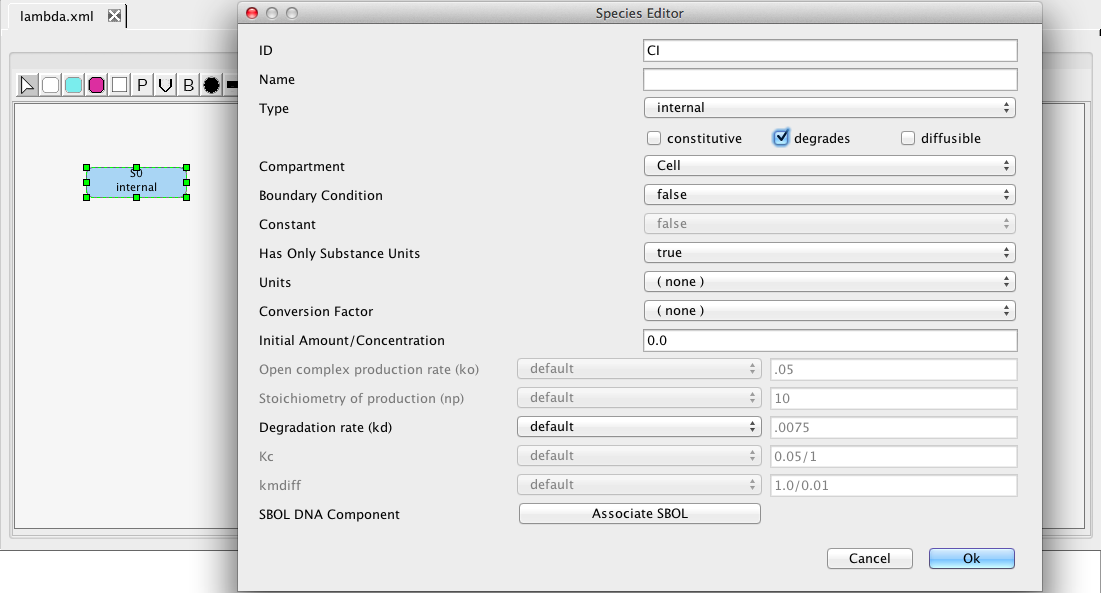
\includegraphics[height=80mm]{screenshots/species}
\end{center}

\subsection{\label{Reactions}Reactions}

\noindent
Reactions are used to create or destroy molecular species in a biochemical reaction network.  
To add a reaction, select the Add Reaction icon 
\includegraphics{../gui/icons/modelview/add_reaction_selected} and click on the schematic canvas which drops a new reaction with a default ID and parameter values.  

\begin{center}
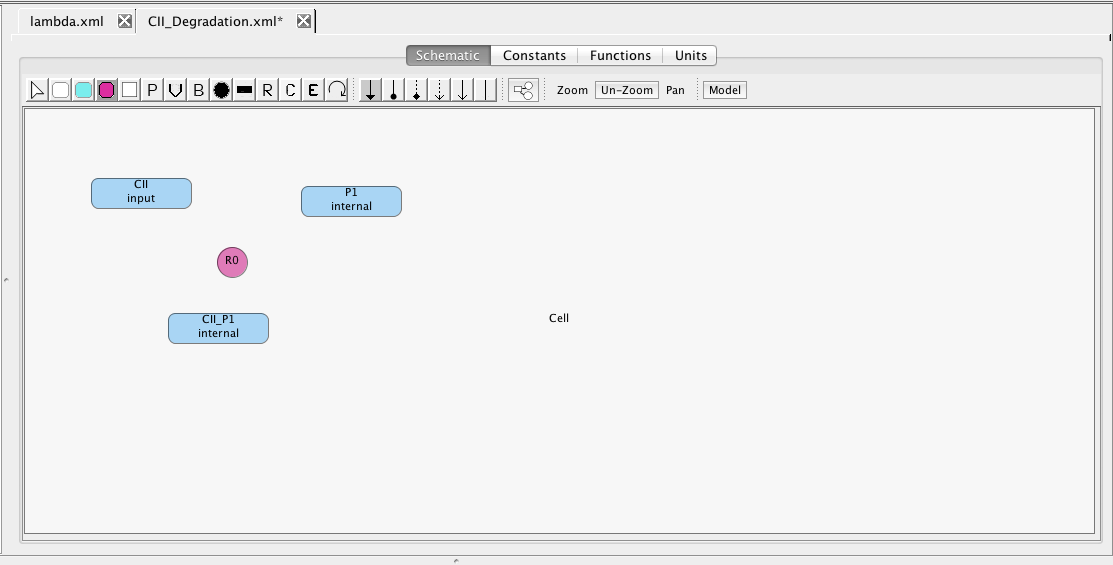
\includegraphics[height=80mm]{screenshots/reaction}
\end{center}

Reactions convert reactant species into product species with perhaps modifier species (e.g., enzymes or catalysts) affecting the rate of this conversion.  The next step, therefore, is to indicate which species are reactants, products, and modifiers for the reaction.  This is accomplished by selecting the Reaction icon 
\includegraphics{../gui/icons/modelview/reaction_selected} or Modifier icon 
\includegraphics{../gui/icons/modelview/modifier_selected}.  With the Reaction icon selected, selecting a species, holding the mouse button, and dragging the arc to a reaction makes the selected species a reactant in that reaction.  Similarly, selecting a reaction, holding the mouse button, and dragging the arc to a species makes the species a product in the selected reaction.  Finally, with the Modifier icon selected, dragging an arc between a species and reaction (in either direction) adds the species as a modifier in the reaction.  When you select a reactant edge, it opens a Reactants Editor.  This editor allows you to change the following things:
\begin{itemize}
\item ID: this is the ID for this reactant and should not be confused with the Species ID.  This ID can be used in equations such as initial, rule, or event assignments.  Use this ID when you want the stoichiometry to be determined by an equation or used in an equation.  The ID is optional.
\item Name: an arbitrary string description of the species (optional).
\item Species: the ID of the reactant species.
\item Stoichiometry: the number of molecules consumed by the reaction.  Note that this value will be overridden when the reactant ID is used on the left-hand side of an assignment.
\item Constant: indicates whether the stoichiometry can change dynamically.  
\end{itemize}
Similarly, the ID, Name, Species, Stoichiometry, and Constant fields can be edited for a Product edge as shown below.  Modifier edges do not have any of these fields, so they cannot be edited.

\begin{center}
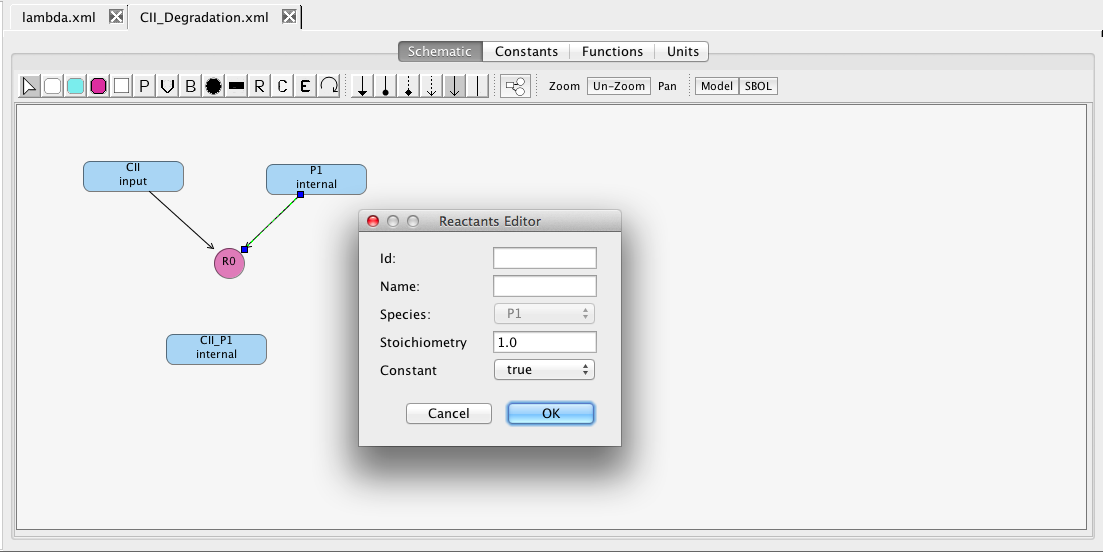
\includegraphics[height=80mm]{screenshots/reactant} 
\end{center}

\begin{center}
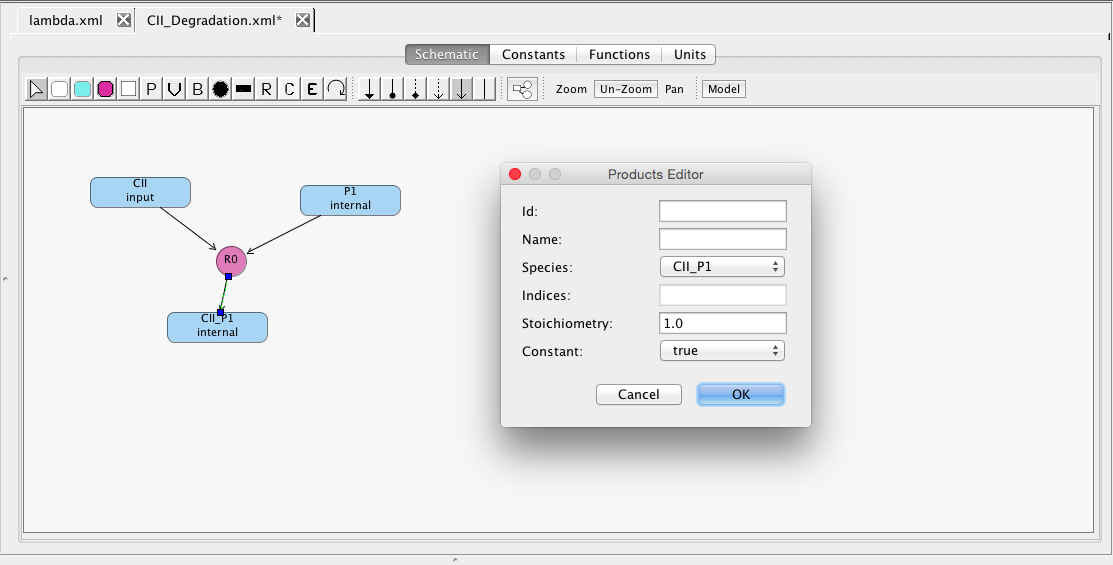
\includegraphics[height=80mm]{screenshots/product}
\end{center}

When you select a reaction, it opens the Reaction Editor which allows you to edit the following reaction fields:
\begin{itemize}
\item ID: a unique ID composed only of alphanumeric characters and underscores.
\item Name: an arbitrary string description (optional).
\item Compartment: the location where this reaction takes place.
\item Reversible: a Boolean indicating if the reaction is reversible (default=false).  Note that reversible reactions are indicated in the schematic with double headed arrows.
\item Fast: a Boolean indicating if the reaction reaches equilibrium rapidly (default=false).  Note that this only has limited support in analysis, so it should be used sparingly.
\item List of Local Parameters: symbolic values that can be used in the \emph{kinetic law} for this reaction.  Their IDs only need to be unique to this reaction.  Local parameters can be added, removed, and edited using the appropriate buttons.  Each parameter is composed of an ID, Name (optional), Value, and Units (optional).  The list of parameters begins with a default forward reaction rate (kf) and reverse reaction rate (kr).  These names and their values should likely be edited. 
\item Kinetic Law: a mathematical formula (see Section~\ref{SBMLMath}) describing the rate or probability for this reaction.  The kinetic law can either be automatically generated using the Use Mass Action button or manually entered.  The Use Mass Action button creates a rate law using the law of mass action assuming that the first parameter in the list is the forward reaction rate and the second parameter in the list is the reverse reaction rate.  
The Clear button clears the kinetic law editor.  Note that the kinetic law formula can only include species IDs that are reactants, products, or modifiers to this reaction.
\end{itemize}

\begin{center}
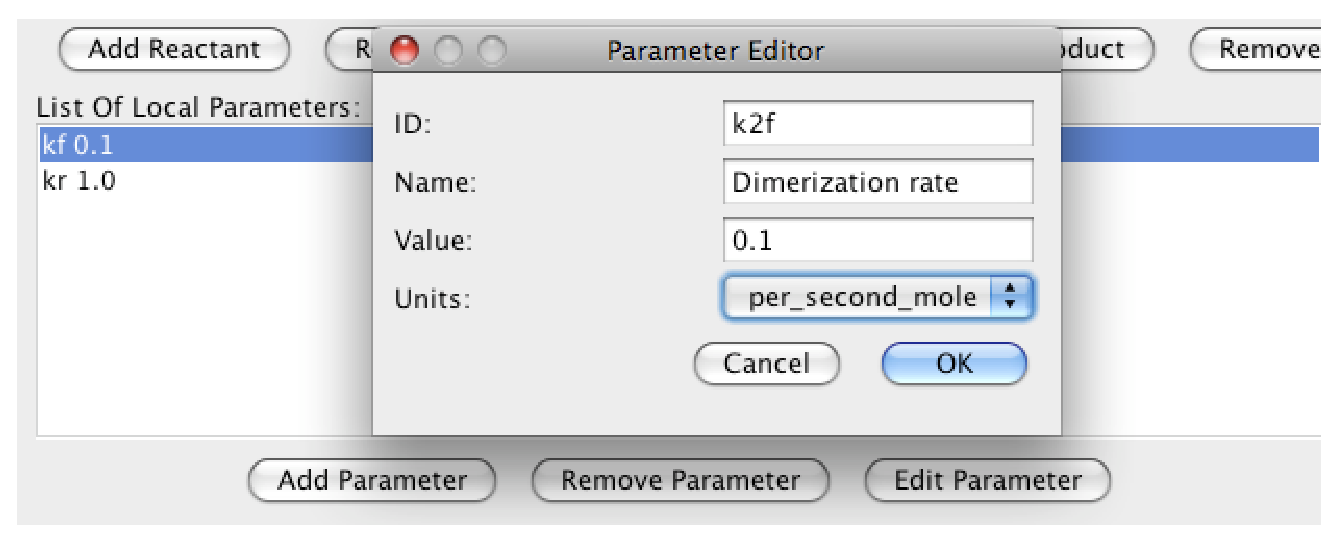
\includegraphics[height=80mm]{screenshots/localParam}
\end{center}

\begin{center}
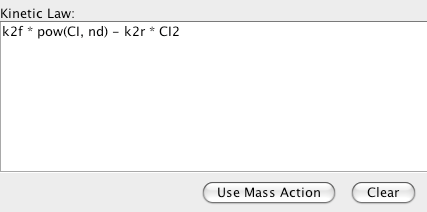
\includegraphics[height=80mm]{screenshots/kineticLaw} 
\end{center}

To simplify a schematic, one can use implicit reactions in some limited situations.  To create an implicit reaction, with the Reaction icon highlighted and the mouse button selected, drag a reaction edge between two species.  This action creates a reaction with a default ID and parameters, including the source species as a reactant and sink species as a product.  If you connect an additional reaction edge to either species, you are asked if you wish to create a new reaction or add this new relationship to an existing reaction on the source and/or sink species.  Implicit reactions can only be used when the following conditions hold:
\begin{itemize}
\item The stoichiometry of all reactants and products for the reaction is 1.
\item The reaction has either a single reactant OR a single product.
\item The reaction has no modifier species.
\end{itemize}
The first condition is a default and cannot be changed.  Adding edges can, however, cause a violation of the second or third condition.  If this violation occurs, an explicit reaction is created to replace the implicit reaction.

\begin{center}
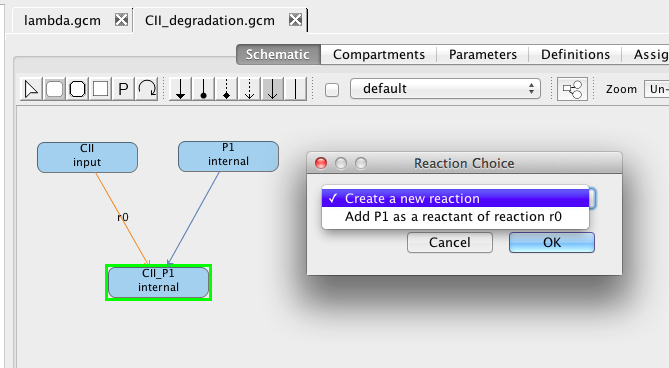
\includegraphics[height=70mm]{screenshots/implicitReactions} 
\end{center}

\subsection{\label{Components}Components}

\noindent
Components are instances of other models within the project, and they are used to create hierarchical, multi-compartment, and cellular population models.  To add a component, select the Add Component icon 
\includegraphics{../gui/icons/modelview/add_component_selected} and click on the schematic canvas.  You are then prompted to select the model for the component that you wish to add.  This window also allows you to add multiple instances of the component at one time.  To do this, select Tile Component and specify how many Columns, Rows, the Padding between them that you want, and whether to start the tiling in the top left corner of the schematic or at the mouse location.  

\begin{center}
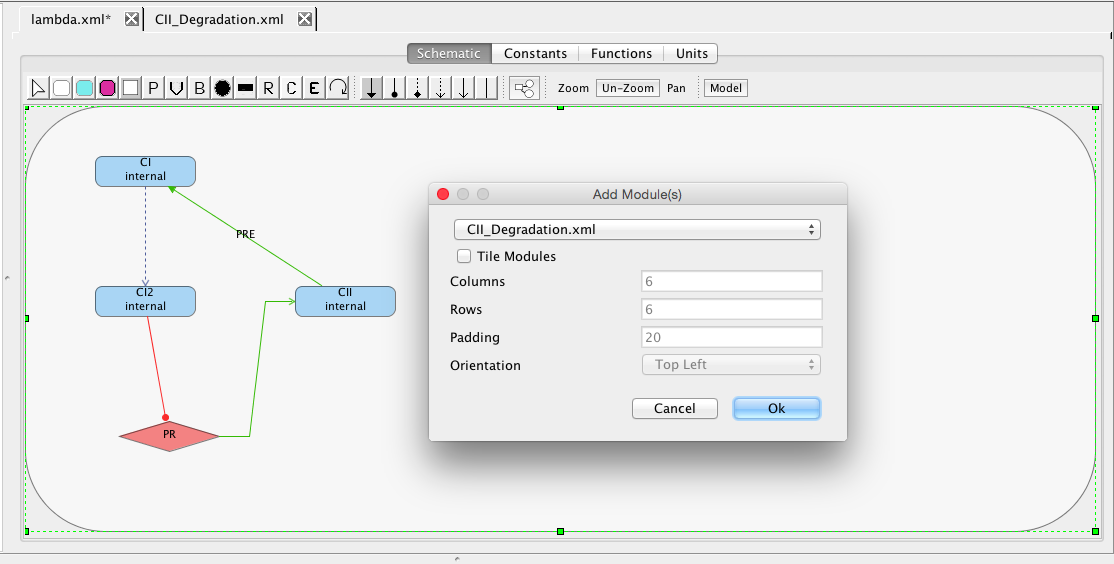
\includegraphics[height=80mm]{screenshots/addComponent}
\end{center}

When a component is added, it appears in the schematic either with sharp or rounded corners.  A component with sharp corners is not enclosed within a compartment, so it may have ports to which species may be connected.  In other words, this is likely part of a hierarchical model.  On the other hand, rounded corners indicate that it is enclosed within a compartment, so it cannot have any ports.  In this case, the component is likely to be part of either a multi-compartment or cellular population model.  If a diffusible species with the same ID exists inside and outside of a compartment-enclosed component, a membrane diffusion reaction will be created, allowing the species to be transported to/from the compartment-enclosed component.  If the compartment-enclosed component is on a grid, the outside diffusible species will be automatically created if the inside diffusible species exists.  Clicking on the component opens the Component Editor, which allows you to change the instance name for the component as well as see a list of the components ports.

\begin{center}
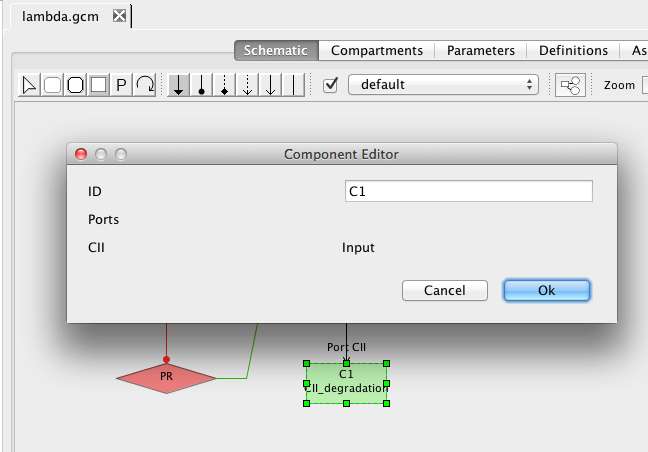
\includegraphics[height=60mm]{screenshots/editComp}
\end{center}

%% TODO: NEED MORE HERE ABOUT WHERE BEHAVIOR IS SPECIFIED

When a component has ports, connections to input ports can be made by selecting a species and, while holding the mouse button, drag an arc to the component.  If there are multiple input ports, you are asked which input port to connect this species to.  To connect to output ports, begin by selecting the component and drag an arc to the species to be connected to the output port.  Note that when you make these connections you are specifying that the species in the top-level model is the same species as the one in the component that it is connected too.  

\begin{center}
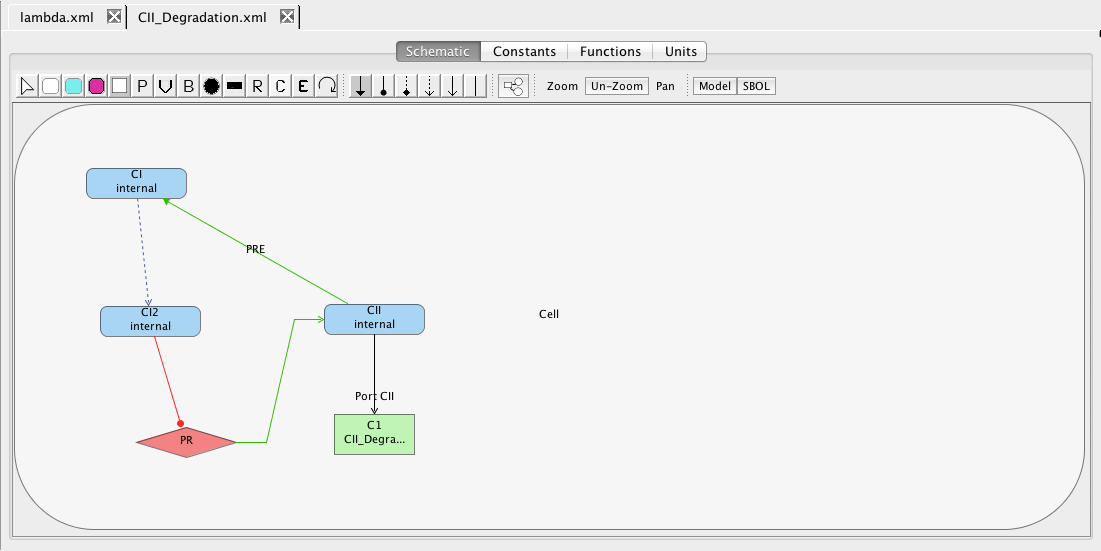
\includegraphics[height=80mm]{screenshots/addPort}
\end{center}

When adding a component to a grid, you are simply asked which model to instantiate, and you cannot connect to ports as species are not allowed on a grid.

\begin{center}
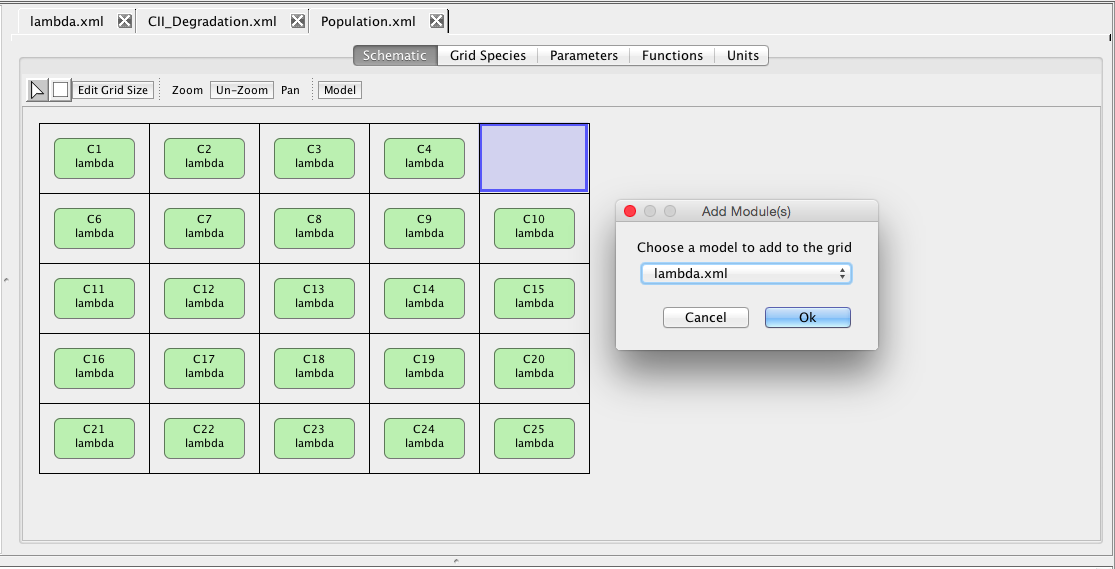
\includegraphics[height=60mm]{screenshots/addCompGrid}
\end{center}

\subsection{\label{Promoters}Promoters}

\noindent
Promoters are the locations on a DNA sequence in which transcription is initiated to create a \emph{messager} RNA (mRNA), which can then be translated by a ribosome into a protein.  To add a promoter to a model, select the Add Promoter icon 
\includegraphics{../gui/icons/modelview/promoter_mode_selected} and click on the schematic canvas, which creates a new promoter with a default ID and parameter values.  Clicking on the promoter opens the Promoter Editor and allows you to edit the following fields:
\begin{itemize}
\item ID: a unique ID composed only of alphanumeric characters and underscores.
\item Name: an arbitrary string description (optional).
\item Initial promoter count (ng): the number of copies of this promoter.  The default is the value of the global parameter ng.   
\item RNAP binding equilibrium (Ko): the equilibrium constant to use for the binding of RNAP to this promoter.  The default value is the global parameter Ko.  Note that this can either be specified as a single equilibrium constant or as a forward rate ``/'' reverse rate.
\item Open complex production rate (ko): once RNAP binds to this promoter, this is the rate at which transcription is initiated.  Note that this production rate is only used for promoters with no activators.  The default value is the global parameter ko.
\item Stoichiometry of production (np): the average number of proteins that are produced by an mRNA before it degrades.  The default value is the global parameter np.
\item Basal production rate (kb): once RNAP binds to an activated promoter, this is the rate at which transcription is initiated without the activator also being bound.  The default value is the global parameter kb.
\item Activated production rate (ka): once RNAP binds to an activated promoter, this is the rate at which transcription is initiated when the activator is also bound to the promoter.  The default value is the global value ka.
\item SBOL Promoter: the DNA component that is associated with this promoter.     Either a full path can be specified (i.e., $\langle$ filename $\rangle$ / $\langle$ collection $\rangle$ / $\langle$ DNA component $\rangle$) or clicking on the Associate SBOL button opens the SBOL browser described in Section~\ref{SBOL}.
\item SBOL Terminator: the DNA component that is associated with the terminator for the transcription initiated by this promoter.     Either a full path can be specified (i.e., $\langle$ filename $\rangle$ / $\langle$ collection $\rangle$ / $\langle$ DNA component $\rangle$) or clicking on the Associate SBOL button opens the SBOL browser described in Section~\ref{SBOL}.
\end{itemize}

\begin{center}
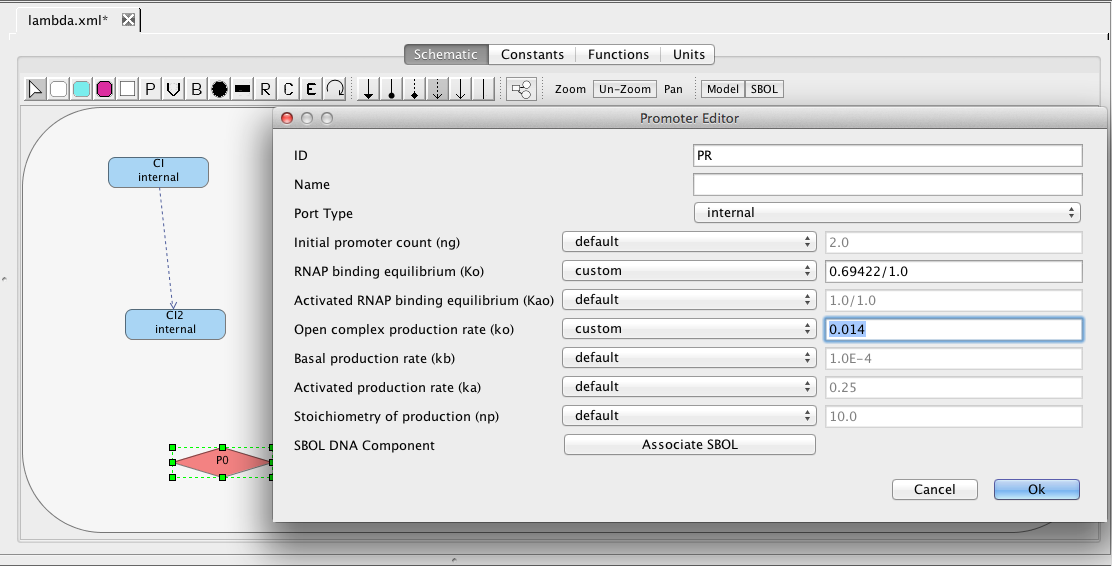
\includegraphics[height=80mm]{screenshots/promoter}
\end{center}

\subsection{\label{Influences}Influences}

There are several types of influences between species that can be specified.  A species may \emph{activate} or \emph{repress} the production of other species.  This relationship is made from a species to the promoter that it activates or represses.  It can also be made directly between two species with an implicit promoter annotating the edge.  One can also specify when there is no influence between two species.  An activating or repressing self-influence can also be specified.  Species can also be related by complex-formation reactions, which indicate that multiple identical or different species can be combined to form a complex species.  

To add a complex-formation reaction, select the complex formation icon 
\includegraphics{../gui/icons/modelview/bio_activation_selected}, highlight a species that is part of a complex, and, while holding the mouse button, stretch the complex formation arc to the complex species.  If you double-click on the complex formation arc, an influence editor will open, which indicates that this is a complex formation arc and the stoichiometry of binding (i.e., the number of molecules of the source species used to construct the sink species) is 2, which you can customize, if desired.

\begin{center}
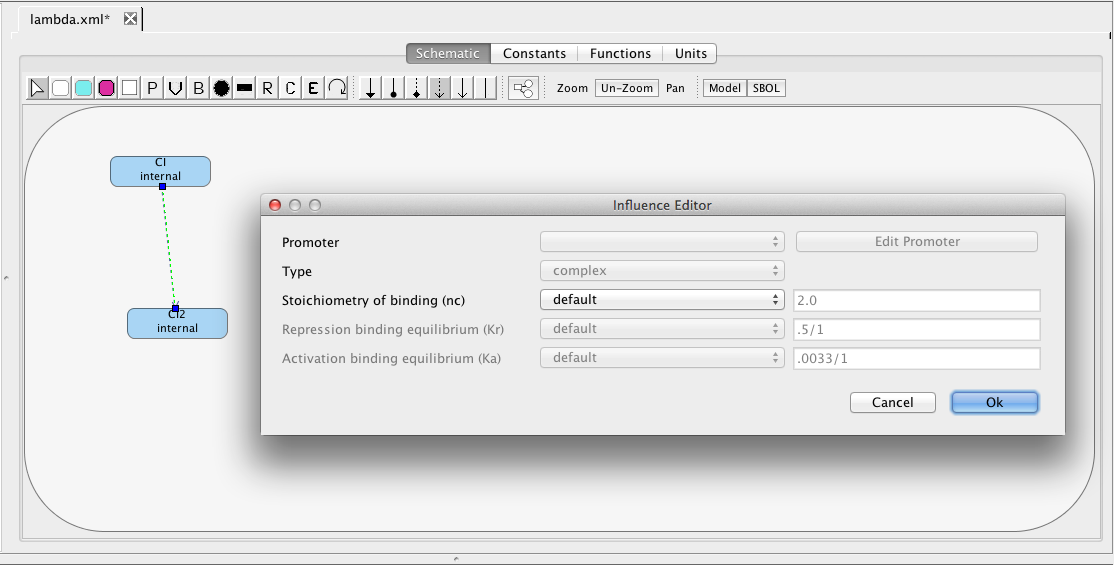
\includegraphics[height=60mm]{screenshots/complex} 
\end{center}

To create a repression influence, select the Repression icon 

\includegraphics{../gui/icons/modelview/inhibition_selected}, highlight the species that is acting as a repressor, and, while holding the mouse button, stretch the repression arc to either the promoter or another species.  In the later, case, an implicit promoter is added.  Double clicking on the repression arc brings up an influence editor.  In this editor, you can customize the stoichiometry of binding as well as the repression binding equilibrium.

\begin{center}
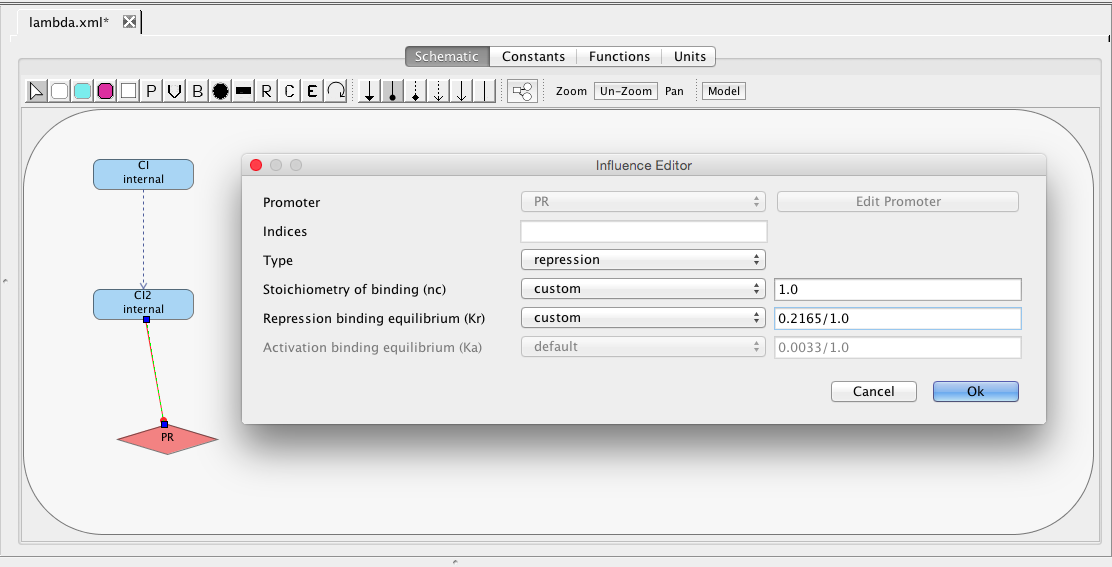
\includegraphics[height=60mm]{screenshots/repression} 
\end{center}

To create an activation influence, select the Activation icon 

\includegraphics{../gui/icons/modelview/activation_selected}, highlight the species that is acting as an activator, and while holding the mouse button stretch the activation arc to either the promoter or another species.  In the latter case, an implicit promoter is added.  Double-clicking on the activation arc brings up an influence editor.  In this editor, you can customize the stoichiometry of binding as well as the activation binding equilibrium.

\begin{center}
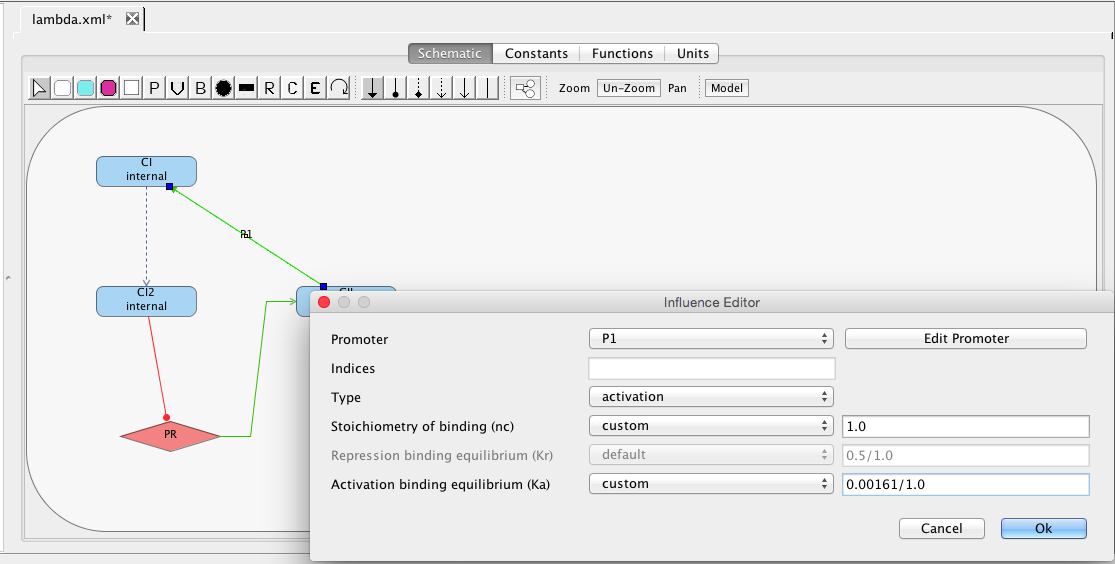
\includegraphics[height=80mm]{screenshots/activation}
\end{center}

To indicate that a species has no influence on another species, select the No Influence icon 

\includegraphics{../gui/icons/modelview/no_influence}, highlight the species that has no influence, and, while holding the mouse button, stretch the no-influence arc to the species it has no influence upon.  Double-clicking on the no-influence arc brings up an influence editor.  In this editor, you can change its type to indicate that it actually has an influence, if you like, and edit accordingly.  No-influence arcs are used by the Learn Tool to avoid adding influences where you are certain there isn't one.

\begin{center}
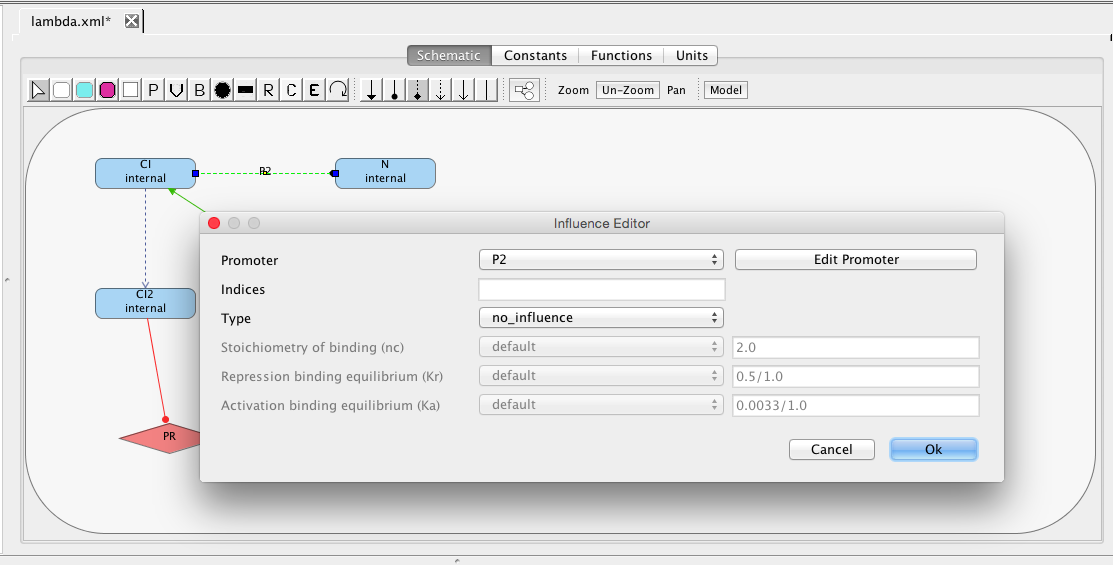
\includegraphics[height=80mm]{screenshots/noInfluence}
\end{center}

The last type of influence is a self-influence.  A self-influence can be either activation or repression.  To create a self-influence, select the Self-influence icon 
\includegraphics{../gui/icons/modelview/self_influence_selected}, select the appropriate Activation or Repression icon, and click on the species that influences itself.  If you click on a self-influence, you will be able to edit its promoter, its type of influence, its stoichiometry of binding, as well as the appropriate binding equilibrium. 

\begin{center}
\includegraphics[height=80mm]{screenshots/selfInfluence}
\end{center}

\subsection{\label{Compartments}Compartments}

\noindent
Compartments are used to specify membrane-enclosed regions where species are found. Every model must include at least one compartment. A new model includes a compartment named {\tt default}.  While its ID and other parameters can be changed, it cannot be removed unless a new compartment is added.  A compartment to which species or reactions have been assigned also cannot be removed.  
As shown below, a compartment has the following fields:
\begin{itemize}
\item ID: a unique ID composed of only alphanumeric characters and underscores.
\item Name: an arbitrary string description (optional).
%\item Type: selected from the list of compartment types (default=none).
\item Dimensions: number of spatial dimensions (default=3).
%\item Outside: the compartment that is outside this compartment  (default=none).
\item Constant: Boolean indicating if the size is constant (default=true).
\item Size: initial size of the compartment (default=1.0).
\item Units: the units for the size (default=none).
\end{itemize}

\begin{center}
\includegraphics[height=80mm]{screenshots/compartment}
\end{center}

\noindent
In addition to the list of compartments, this tab also includes the Model ID (which cannot be changed), the Model Name (an arbitrary string description of this model), and the Model Units.  Clicking on the Model Units button allows you to see and edit this model's default units.  The substance units are the default units for species, the time units are the default units for time, the volume units are the default units for 3-dimensional compartments, the area units are the default units for 2-dimensional compartments, the length units are the default units for 1-dimensional compartments, the extent units are the defaults units for the amount changed due to a reaction.  Kinetic laws have default units of extent units / time units.  The conversion factor is the constant global parameter to be used as the default conversion factor to convert species units into extent units.

\begin{center}
\includegraphics[height=80mm]{screenshots/ModelUnits}
\end{center}

\subsection{\label{Parameters}Parameters}

\noindent
There are two types of parameters: model generation parameters and global parameters.  The model generation parameters provide default parameter values when converting a model into a reaction-based model for analysis. 
In the Species, Promoter, and Influence Editors, any parameter set to default uses the value found in this list.  These defaults can be modified in the user preferences (see Section~\ref{Preferences}).  The user can also edit these parameters for an individual model by changing the default to custom, then changing the value.

\begin{center}
\includegraphics[height=80mm]{screenshots/GCMparam}
\end{center}

%% TODO: update this list
% The complete list of Model Generation Parameters are listed below:

% \begin{center}
% \begin{tabular}{|c|c|c|c|c|}
% \hline
% ID & Default Value & Units      & Structure & Description \\ \hline \hline
% nr & 30            & molecule   & model     & Initial RNAP count \\ \hline
% ns & 0             & molecule   & species   & Initial species count \\ \hline
% Kd & 0.05          & $\frac{1}{\mathrm{molecule}}$ & species   
% & Dimerization equilibrium\\ \hline
% kd & 0.0075        & $\frac{1}{\mathrm{sec}}$ & species   
% & Degradation rate \\ \hline
% ng & 2             & molecule   & promoter  & Initial promoter count \\ \hline
% np & 10            & molecule   & promoter  & Stoichiometry of
% production \\ \hline
% nc & 2             & molecule   & promoter  & Degree of cooperativity \\ \hline
% Ko & 0.033         & $\frac{1}{\mathrm{molecule}}$ & promoter  
% & RNAP binding equilibrium\\ \hline
% ko & 0.05          & $\frac{1}{\mathrm{sec}}$ & promoter  
% & Open complex production rate \\ \hline
% kb & 0.0001        & $\frac{1}{\mathrm{sec}}$ & promoter  
% & Basal production rate \\ \hline
% ka & 0.25          & $\frac{1}{\mathrm{sec}}$ & promoter  
% & Activated production rate\\ \hline
% nd & 1             & molecule   & influence & N-mer as transcription
% factor \\ \hline
% Kr & 0.5           & $\frac{1}{\mathrm{molecule}^{nc}}$ & influence
% & Repression binding equilibrium \\ \hline
% Ka & 0.0033        & $\frac{1}{\mathrm{molecule}^{(nc+1)}}$ & influence
% & Activation binding equilibrium \\ \hline
% Kb & 0.05          & $\frac{1}{\mathrm{molecule}}$ & influence
% & Biochemical equilibrium \\ \hline
% \end{tabular}
% \end{center}

\noindent
Global Parameters are variables that can be used in math formulas (see Section~\ref{SBMLMath}).  A parameter includes the following:
\begin{itemize}
\item ID: a unique ID composed only of alphanumeric characters and underscores.
\item Name: an arbitrary string description (optional).
\item Value: initial value for the parameter.
\item Units: the units for the parameter value (default=none).
\item Constant: Boolean indicating if the parameter value is constant (default=true).
\end{itemize}

\begin{center}
\includegraphics[height=80mm]{screenshots/parameter}
\end{center}

\subsection{\label{Definitions}Definitions}

\noindent
The Definitions tab allows users to provide function and unit definitions. Function definitions are used to create user-defined functions that can then be used in math formulas (see Section~\ref{SBMLMath}).  As shown below, function definitions include an ID, an optional name field, a comma-separated list of arguments, and its definition.  The definition is a math formula, though it is restricted to the use of variable names which are arguments to the function.  While functions can call other functions, they cannot be recursive (i.e., call themselves) either directly or indirectly (i.e., through a cycle of function calls).  Several random functions supported by {\tt iBioSim}'s simulators are added automatically to every model.

\begin{center}
\includegraphics[height=80mm]{screenshots/function}
\end{center}

\noindent
Unit definitions are used to construct user-defined units which are derived from the set of base units.  As shown below, a unit definition includes an ID, an optional name, and a list of units that define it.  There are buttons to add, remove, and edit elements in the list of units.  Each unit is composed of a kind, exponent, scale, and multiplier.  The kind is selected from the list of base units in the table below.  The exponent and multiplier are real numbers, and the scale is an integer that specifies the relationship between the derived unit and the base unit using the relation below:
\begin{eqnarray*}
\mathrm{unit} & = & (\mathrm{multiplier} * 10^\mathrm{scale} * \mathrm{baseUnit})^\mathrm{exponent}
\end{eqnarray*}

\begin{center}
\includegraphics[height=80mm]{screenshots/units}
\end{center}

\begin{center}
\begin{tabular}{|c|c|c|c|c|c|}
\hline
ampere        & farad  & joule    & lux  & radian    & volt \\ \hline
avogadro     & gram  & katal   & metre   & second   & watt \\ \hline
bacquerel       & gray & kelvin & mole & siemens   & weber \\ \hline
candela       & henry & kilogram    & newton    & sievert & ~\\ \hline
coulomb & hertz  & litre    & ohm & steradian     & ~\\ \hline
dimensionless         & item & lumen      & pascal & tesla      & ~\\ \hline
\end{tabular}
\end{center}

% \subsubsection{\label{compTypes}Compartment Types}

% \noindent
% Compartment types are used to relate multiple compartments.  As shown
% below, a compartment type includes an ID and an optional name field.
% \begin{center}
% \includegraphics[height=50mm]{screenshots/compType}
% \end{center}

% \subsubsection{\label{specTypes}Species Types}

% \noindent
% Species types are used to relate multiple species.  As shown below, a 
% species type includes an ID and an optional name field.
% \begin{center}
% \includegraphics[height=50mm]{screenshots/specType}
% \end{center}

\subsection{\label{Assignments}Assignments}

\noindent
There are two types of assignments: initial assignments and rules.  Initial assignments as shown below are used to provide a mathematical formula (see Section~\ref{SBMLMath}) that is evaluated at time 0 to determine the initial value of a compartment size, species amount or concentration, or parameter.  The value of this formula takes precedence over the initial value specified in the object.  

\noindent
There are three types of rules: algebraic, assignment, and rate rules:
\begin{center}
\begin{tabular}{|c|c|c|}
\hline
Algebraic  & left-hand side is zero             & $0 = f(W)$ \\ \hline
Assignment & left-hand side is a scalar         & $x = f(W)$ \\ \hline
Rate       & left-hand side is a rate-of-change & $\frac{dx}{dt} = f(W)$ 
\\ \hline
\end{tabular}
\end{center}

\begin{center}
\includegraphics[height=80mm]{screenshots/initial}
\end{center}

\noindent
Algebraic rules specify relationships which must be maintained.  Assignment rules specify the value of a compartment size, species amount or concentration, or parameter in terms of a mathematical formula (see
Section~\ref{SBMLMath}).  A variable cannot be determined by both an assignment rule and initial assignment.  Rate rules specify the rate of change of a compartment size, species amount or concentration, or parameter in terms of a mathematical formula (see Section~\ref{SBMLMath}).  A variable cannot be determined by both an assignment rule and a rate rule.  A species that is a reactant or a product of any reaction cannot be updated by either an assignment rule or rate rule.  
When adding a rule, the user first selects the type of rule as shown below.  This automatically restricts the set of variables available for the left-hand side to those that are valid.  The user should then select a variable (except in the case of an algebraic rule) and enter a mathematical formula (see Section~\ref{SBMLMath}) for the rule.  When editing a rule, the user cannot modify the rule type. 

\begin{center}
\includegraphics[height=80mm]{screenshots/rule}
\end{center}

\subsection{\label{Properties}Properties}

The properties tab allows users to provide formulas for either desired or un-desired behavior.  These formulas can be provided in two forms as either a \emph{Continuous Stochastic Logic} (CSL) property (see Section~\ref{CSL}) or as a constraint.  CSL is a temporal logic which allows one to specify probabilistic temporal logic properties.  Analysis of a CSL property should return the probability that the property is true.  These properties can either be transient properties to ask if something happens within a certain amount of time, or steady-state properties to ask the probability of a given state as time goes to infinity.  The syntax for our CSL properties is given in Section~\ref{CSL}.

\begin{center}
\includegraphics[height=80mm]{screenshots/properties}
\end{center}

\noindent
Constraints are used to specify properties that should cause simulation to terminate.  As shown below, each constraint is composed of an ID which is used to identify it in graphs, a constraint given as a mathematical formula (see Section~\ref{SBMLMath}), and a message describing the constraint.  A default ID is automatically generated when a new constraint is created.

\begin{center}
\includegraphics[height=80mm]{screenshots/constraint}
\end{center}

Our analysis methods can provide histograms that show the proportion of simulations that either satisfy a CSL property or are terminated due to a constraint.  Analysis can also show time-series plots showing the proportion of simulations at each time point that have either satisfied a CSL property or terminated due to a constraint. 

\subsection{\label{Events}Events}

\noindent
Events are used to specify discrete changes of compartment sizes, species amounts or concentrations, and parameter values.  Each event is composed of the following items:
\begin{itemize}
\item ID: a unique ID composed only of alphanumeric characters and underscores.
\item Name: an arbitrary string description (optional).
\item Trigger: a mathematical formula which, when it changes evaluation from false to true, indicates that the event is triggered.
\item Delay: a mathematical formula which is evaluated when an event is triggered, and the result is the amount of time before the event is to be executed.
\item Priority: a mathematical formula which sets the priority for this event when multiple events are scheduled to be executed simultaneously.  In this situation, the event with the highest priority is the next to be executed.
\item Use values at trigger time: this Boolean indicates if values for the event assignments should be calculated at trigger time or execution time (default=false).
\item Trigger is persistent: this Boolean indicates the behavior when a trigger expression becomes false before an event is executed.  If it is persistent, then it still executes when ready.  If it is not persistent, then the event is disabled and no longer scheduled to execute (default=false).
\item Trigger is initially true: this Boolean indicates the behavior when a trigger evaluates to true at time 0.  If it is initially true, there is no change in evaluation, so the event is not triggered.  If it is not initially true, there is now a change in evaluation, so the event is triggered.
\item List of Event Assignments: these indicate how the state is supposed to change when the event executes.  Use the add, remove, and edit assignment buttons to update them.  In the event assignment editor, the variable to change must be selected and the assignment to be performed must be specified as a mathematical formula.
\end{itemize}

\begin{center}
\includegraphics[height=80mm]{screenshots/event}
\end{center}

\clearpage

\section{\label{SBOL}SBOL Browser}

SBOL is an emerging standard under development for the exchange of information about synthetic biology designs.  An SBOL file includes \emph{Collections} of \emph{DNA Components}.  Each DNA component has a unique ID, name, description, type, and a DNA sequence.  A DNA component can be a simple sequence feature like a promoter, ribosome binding site, open reading frame (i.e., gene), or terminator.  It can also be an annotated DNA sequence that includes several of these individual features, perhaps organized hierarchically.  For example, a DNA component may include a promoter followed by a ribosome binding site followed by an open reading frame followed by a terminator.  {\tt iBioSim} includes an SBOL browser that allows the user to view an individual SBOL file by clicking on it in the list of project files.  In this browser, you can highlight individual DNA components and see the information stored about them.

\begin{center}
\includegraphics[height=80mm]{screenshots/SBOLBrowser}
\end{center}

A similar SBOL browser is available for associating DNA components to a model.  Namely, for a promoter, you can associate both a DNA component to the promoter as well as a terminator for the transcription initiated at this promoter.  For a species, you can associate both a DNA component for the open reading frame for the gene that produces this species as well as the ribosome binding site where translation begins for this gene.  This SBOL browser is opened by clicking on an Associate SBOL button within either the Species Editor (see Section~\ref{Species}) or Promoter Editor (see Section~\ref{Promoters}).  This browser only shows DNA components of the appropriate type.  For example, when associating a species to its open reading frame, only DNA components of the open reading frame type are shown.

\begin{center}
\includegraphics[height=80mm]{screenshots/AssociateSBOL}
\end{center}

%% TODO: ADD LPN EDITOR

% \section{\label{LPNEdit}LPN Model Editor}

% NEED STUFF HERE

% \subsection{\label{Variables}Variables}

% NEED STUFF HERE

% \subsection{\label{Places}Places}

% NEED STUFF HERE

% \subsection{\label{Transitions}Transitions}

% NEED STUFF HERE

% \subsection{\label{ControlFlow}Control Flow}

% NEED STUFF HERE

% \subsection{\label{LPN Properties}Properties}

% NEED STUFF HERE

\clearpage

\section{\label{Analysis}Analysis Tool}

\noindent
The analysis tool is used to analyze biochemical reaction network models.  {\tt iBioSim} comes with a number of simulation methods, ranging from continuous-deterministic (ODE) simulation methods to discrete-stochastic (Monte Carlo) simulation methods.  In order to perform efficient temporal behavior analysis, various model abstractions can also be automatically applied.  Many of the analysis and abstraction routines are implemented
within the reb2sac tool described in 
%%tth:\begin{html}<A HREF="http://www.async.ece.utah.edu/publications">\end{html}
Kuwahara's PhD Dissertation (UofUtah 2007).
%%tth:\begin{html}</A>\end{html}
  An analysis view includes several tabs.  The Simulation Options tab, described in Section~\ref{simOptions}, selects the different simulation methods and parameters.  The Abstraction Options tab described in Section~\ref{absOptions} configures model abstraction.  The Schematic tab, described in Section~\ref{AnalysisSchematic}, allows the user to modify or sweep various parameters on the schematic.  It also provides an alternative way of visualizing simulation data upon the schematic.  The Parameters tab allows the user to modify or sweep model generation and global parameters, and it is described in Section~\ref{AnalysisParameters}.  The SBML elements tab described in Section~\ref{SBMLElements} allows the user to add or remove parts of the model during analysis.  The TSD Graph tab is a graph editor for some series data, and it is described in Section~\ref{TSDGraph}.  Finally, the Histogram tab is a graph editor for probability data, and it is described in Section~\ref{Histogram}.

\begin{center}
\includegraphics[height=90mm]{screenshots/analysisView}
\end{center}

\subsection{\label{simOptions}Simulation Options}

\noindent
The first set of radio buttons in this tab specifies the type of abstraction. 
\begin{itemize}
\item None: use no abstraction.
\item Abstraction: perform reaction-based abstraction.
\item Logical Abstraction: perform both reaction-based and logical abstractions.
\end{itemize}

\noindent
The second set of radio buttons specify the type of analysis.  
\begin{itemize}
\item ODE: continuous-deterministic simulation.
\item Monte Carlo: discrete-stochastic simulation.
\item Markov: performs temporal probability distribution analysis on finite-state Markov chain models (this requires logical abstraction).
\item Model: produces a flattened model and puts it in the list of project files.
\item Network: outputs the model in the GraphViz format for display by dotty.
\item Browser outputs the model in xhtml format for display in a web browser.
\item LPN: produces an LPN model and puts it in the list of project files (this requires logical abstraction).  
\end{itemize}
Some results selecting Model, Network, and Browser are shown below.

\begin{center}
\includegraphics[height=80mm]{screenshots/reactionModel}
\end{center}

\begin{center}
\includegraphics[height=80mm]{screenshots/viewNetwork}
\end{center}

\begin{center}
\includegraphics[height=110mm]{screenshots/viewBrowser}
\end{center}

\noindent
The next group of options are for simulation-based analysis only.
\begin{itemize}
\item Report concentrations: if checked, report concentrations rather than amounts (default=amounts).
\item Do Not Generate Runs: if checked, simulation data is not produced, though summary probabilistic data is still produced (default=Generate Runs).
\item Append Simulation Runs: if checked, additional simulation runs are added to the existing set of simulation runs rather than first removing the previous runs (default=overwrite).  Note that the seed changes automatically when this gets checked, because otherwise the additional runs will likely be the same as the previous set.
\end{itemize} 

\noindent
The next field specifies the simulation method you want to use based on the simulation type you specified. The methods available are:
\begin{center}
\begin{tabular}{|c|c|l|}
\hline
Type & Method ID & Description \\ \hline \hline
ODE  & Euler     & The forward Euler Method \\ \hline
ODE  & gear1     & Gear Method M=1 \\ \hline
ODE  & gear2     & Gear Method M=2 \\ \hline
ODE  & rk4imp    & Implicit 4th order Runge-Kutta at Gaussian points \\ \hline
ODE  & rk8pd     & Embedded Runge-Kutta Prince-Dormand (8,9) method \\ \hline
ODE  & rkf45     & Embedded Runge-Kutta-Fehlberg (4, 5) method \\ \hline
Monte carlo & Gillespie & Gillespie's SSA direct method \\ \hline 
Monte carlo & GillespieJava & Java implementation of Gillespie's SSA direct method \\ \hline  
Monte carlo & mpde & iSSA using marginal probability density evolution \\ \hline   
Monte carlo & mp & iSSA using the mean path \\ \hline    
Monte carlo & mp-adaptive & iSSA using the mean path and adaptive step size\\ \hline     
Monte carlo & mp-event & iSSA using the mean path and event count step size \\ \hline     
Monte carlo & emc-sim   & Use jump count as next reaction time \\ \hline
Monte carlo & bunker    & Uses mean for next reaction time \\ \hline
Monte carlo & nmc       & Uses normally distributed next reaction time \\ \hline
Markov & steady-state & Steady-state Markov chain analysis \\ \hline
Markov & transient & Transient Markov chain analysis \\ \hline
Markov & reachability & Only perform reachability analysis \\ \hline
Markov & atacs & Use {\tt atacs} steady-state Markov analysis engine \\ \hline
Markov & ctmc-transient & Transient distribution analysis \\ \hline
\end{tabular}
\end{center}

There are some properties that need to be set for simulation.
The table below specifies these:

\begin{center}
\begin{tabular}{|l|l|}
\hline
Field             & Description \\ \hline \hline
Time Limit        & The simulation time limit \\ \hline
Choose one:    &  \\ \hline
~~~Print Interval    & The print time interval for each simulation run \\ \hline 
~~~Minimum Print Interval    & Print on change but no more often than this interval \\ \hline  
~~~Number of Steps    & Number of steps to print \\ \hline  
Minimum Time Step & The smallest time step allowed \\ \hline
Maximum Time Step & The largest time step allowed \\ 
      ~           & (also the time step used for the Euler method) \\ \hline
Absolute Error    & Used by the adaptive time step ODE methods \\ \hline
Random Seed       & An integer number as a seed to generate random numbers \\ \hline
Runs              & The number of random simulation runs to perform \\ \hline
Simulation ID     & Creates a simulation directory with the ID name \\ \hline
\end{tabular}
\end{center}

\subsection{\label{absOptions}Abstraction Options}

\noindent
Abstraction is performed in three steps.  There is a preprocess step, which is a sequence of abstractions performed once on the initial model.  The main loop iterates through a group of abstractions until there is no change in the model.  Finally, there is a postprocess step, which is a sequence of abstractions performed once at the end.  Clicking on the Add button brings up a list of all the possible abstraction methods.  The selected abstraction method is added after the highlighted abstraction method in the list.  If no method is highlighted, it makes it the first abstraction in the list.

\begin{center}
\includegraphics[height=80mm]{screenshots/absOptions}
\end{center}

{\tt iBioSim} supports many different types of abstraction.  However, there are a few critical ones that we list here:
\begin{itemize}
\item complex-formation-and-sequestering-abstraction: this attempts to remove complex formation reactions.  It replaces the complex species in rate laws with a function of its constituent species.
\item operator-site-reduction-abstraction: this removes reactions and corresponding species involved in the binding of transcription factors to operator sites.
\item distribute-transformer: applies the distributive law to kinetic law formulas to make it easier to identify the forward and reverse rates within a reversible reaction.
\item reversible-to-irreversible-transformer: this converts a reversible reaction into two irreversible reactions.  This is critical for the Monte Carlo simulation methods that require there to be no reversible reactions.
\item kinetic-law-constants-simplifier: this replaces constant parameters within kinetic laws with their values to improve their evaluation time.
\end{itemize}

\noindent
This tab also includes a few parameters for the abstraction methods.
\begin{itemize}
\item Rapid Equilibrium Condition 1 specifies threshold T1 such that the rapid equilibrium condition fails when $T1 > E0 / (S0 + k-1/k1)$.
\item Rapid Equilibrium Condition 2 specifies threshold T2 such that the rapid equilibrium condition fails when $T1 > k2 /k-1$.
\item The QSSA condition specifies threshold T used by the QSSA abstraction method where $T > E0 / (S0 + KM)$.
\item The Max concentration threshold specifies the maximum number of molecules that a species can have initially and still be considered an operator site by the operator site reduction. 
\end{itemize}
Note that these are not used by the common abstractions listed above.

% Here, you can specify additional options for your analysis.
% For each option, you must provide the name of the option and its
% value. 
% % <!-- For example, property
% % <I>reb2sac.abstraction.method.1.x</I>&nbsp; specifies a list of
% % abstraction methods used for pre-processing, property
% % <I>reb2sac.abstraction.method.2.x </I>specifies a list of
% % abstraction methods used in the main abstraction loop, and&nbsp;
% % property <I>abstraction.method.3.x</I> is a list of abstraction
% % methods used for post-processing.&nbsp; These abstraction method
% % properties can take the following values: 
% % 
% % \begin{itemize}
% % <LI><P STYLE="margin-bottom: 0in">modifier-structure-transformer
% % 
% % <LI><P STYLE="margin-bottom: 0in">modifier-constant-propagation 
% % 
% % <LI><P STYLE="margin-bottom: 0in">operator-site-forward-binding-remover
% % 
% % <LI><P STYLE="margin-bottom: 0in">nary-order-unary-transformer2 
% % 
% % <LI><P STYLE="margin-bottom: 0in">kinetic-law-constants-simplifier
% % 
% % <LI><P STYLE="margin-bottom: 0in">enzyme-kinetic-rapid-equilibrium-1
% % 
% % <LI><P STYLE="margin-bottom: 0in">dimer-to-monomer-substitutor 
% % 
% % <LI><P STYLE="margin-bottom: 0in">dimerization-reduction 
% % 
% % <LI><P STYLE="margin-bottom: 0in">kinetic-law-constants-simplifier
% % 
% % <LI><P STYLE="margin-bottom: 0in">irrelevant-species-remover 
% % 
% % <LI><P STYLE="margin-bottom: 0in">inducer-structure-transformer 
% % 
% % <LI><P STYLE="margin-bottom: 0in">final-state-generator 
% % 
% % <LI><P STYLE="margin-bottom: 0in">similar-reaction-combiner 
% % 
% % <LI><P STYLE="margin-bottom: 0in">absolute-inhibition-generator 
% % 
% % <LI><P STYLE="margin-bottom: 0in">reversible-to-irreversible-transformer
% % 
% % <LI><P STYLE="margin-bottom: 0in">multiple-products-reaction-eliminator
% % 
% % <LI><P STYLE="margin-bottom: 0in">multiple-reactants-reaction-eliminator
% % 
% % <LI><P STYLE="margin-bottom: 0in">single-reactant-product-reaction-eliminator
% % 
% % <LI><P STYLE="margin-bottom: 0in">stop-flag-generator 
% % 
% % <LI><P STYLE="margin-bottom: 0in">enzyme-kinetic-qssa-1 
% % 
% % <LI><P STYLE="margin-bottom: 0in">birth-death-generator4 
% % 
% % <LI><P STYLE="margin-bottom: 0in">max-concentration-reaction-adder
% % 
% % \item dummy-abstraction-method 
% % 
% % \end{itemize}
% % <P>
% % -->
% On this tab, there are buttons to add a new option, edit an
% existing option, remove an existing option, or clear all options.

\subsection{\label{AnalysisSchematic}Schematic}

\noindent
Using the schematic tab, you can adjust initial values and parameters, allowing one to perform simulations to determine the effect of these changes.  Clicking on any species, promoter, reaction, or influence brings up the corresponding editor.  To change a value, switch the corresponding combo box to modified, which will then allow you to change the value.  

\begin{center}
\includegraphics[height=50mm]{screenshots/paramEdit}
\end{center}

In addition to making single changes, you can also sweep a value as shown below.  When you click on the Sweep button, it brings up a window where you can select the start value, the stop value, and the step value.  The level indicates how the sweep should perform when multiple variables are swept at the same time.  Variables at the same level are changed at the same time.  Furthermore, all variables on level 2 are stepped through all their values before changing the values of those variables on level 1.  After the values on level 1 are changed, the values on level 2 are stepped through all their values again.  

\begin{center}
\includegraphics[height=50mm]{screenshots/sweep}
\end{center}

The schematic tab can also be used to visualize simulation results.  To do this, after you have generated some simulation results, you can press the Choose Simulation button to bring up a window with all the simulations in this analysis view.  You can then select the data that you would like to visualize.

\begin{center}
\includegraphics[height=80mm]{screenshots/chooseSim}
\end{center}

If you now click on a species, component, or grid location, you can modify how it appears as you playback the simulation.  You can have it change color, size, and/or opacity on a gradient.  You can also select the range of molecule counts to specify the ends of the gradient(s).  Finally, you can indicate that these selections are either for this species or all species in the model.  Appearances can be saved by clicking the save button.

\begin{center}
\includegraphics[height=50mm]{screenshots/editSpeciesAppearance}
\end{center}

The appearances editor for components and grid locations is similar.  The differences are that you can select any species within the component (or diffusible species for the grid location).  You also can copy the settings to all instantiations of the same model.

\begin{center}
\includegraphics[height=80mm]{screenshots/compAppearances}
\end{center}

Once you have made your selections, you can now playback the simulation.  You can either single-step the simulation by pressing the \includegraphics{../gui/icons/modelview/movie/single_step} icon or play continuously by pressing the \includegraphics{../gui/icons/modelview/movie/play} icon.  The playback can also be paused by pressing the \includegraphics{../gui/icons/modelview/movie/pause} icon and restarted by pressing the  \includegraphics{../gui/icons/modelview/movie/rewind} icon.  The slider can be dragged around to quickly reach a particular spot in simulation

\begin{center}
\includegraphics[height=80mm]{screenshots/movieView}
\end{center}

\clearpage

\subsection{\label{AnalysisParameters}Parameters}

\noindent
The parameter tab allows the user to modify the value of any model generation or global parameter for a given analysis.  Like the values on the schematic tab, they can also be swept to generate multiple simulation runs stepping through different values.

\begin{center}
\includegraphics[height=80mm]{screenshots/parameterEditor}
\end{center}

\subsection{\label{SBMLElements}SBML Elements}

\noindent
The SBML elements tab allows you to select which SBML model elements to include in your analysis.  This includes initial assignments, rules, constraints, and events.  Elements that are checked are used during analysis.  Otherwise, they are not used.

\begin{center}
\includegraphics[height=80mm]{screenshots/SBMLElements}
\end{center}

\clearpage

\section{\label{Learn}Learn Tool}

\noindent
The Learn Tool is used to discover genetic circuit connectivity from time series data.  This tool uses the GeneNet algorithm described in
%%tth:\begin{html}<A HREF="http://www.async.ece.utah.edu/publications">\end{html}
Barker's PhD dissertation (University of Utah 2007).
%%tth:\begin{html}</A>\end{html}
  The first tab of the Learn Tool is the \emph{data manager} which is shown below.  It is used to both enter time series experimental data as well as bring data into the learn view.  The Add button is used to create a new data file. After pressing this button, enter the name of the new data file, and then enter the data for this file using the data editor to the right.  The Remove button deletes all highlighted files.  Note that after highlighting one file, you can use the ctrl key to highlight additional files or the shift key to highlight a range of files.  The Rename button is used to change the name of a data file. The Copy button copies a data file. The Copy From View button brings up a list of all analysis and learn views in the current project, and data from the selected view will be copied into this learn view.  Finally, the Import button brings up a file browser, and it allows you to import a data file from outside
this project.  These files can be in time series data (TSD) format (see Section~\ref{TSD}), comma separated value (CSV) format, or tab delimited format (DAT).  
The contents of the data file highlighted on the left appear in the data editor on the right.  Individual data entries can be modified, new data points can be added using the Add Data Point button, data points can be removed using the Remove Data Point button, and data points can be copied using the Copy Data Point button.  When you are
satisfied with all your changes, you should press the Save button to record your changes.

\begin{center}
\includegraphics[height=80mm]{screenshots/dataManager}
\end{center}

\noindent
The second tab allows the user to configure the basic options for the Learn Tool.  The basic options include:
\begin{itemize}
\item Minimum Number of Initial Vectors (Tn) (default=2): \\
Tn is a threshold value used in the CreateInfluenceVectorSet algorithm and represents the minimum number of influence vectors constructed in this algorithm.
\item Maximum Influence Vector Size (Tj) (default=2): \\
Tj is a threshold value used in the CombineInfluenceVectors algorithm to determine the maximal size of merged influence vectors.
\item Score for Empty Influence Vector (Ti) (default=0.5): \\
The score for an influence vector with no influences in it.
\item Number of Bins (default=4): \\
The number of bins value specifies how many values the encoded time series data can assume.
\item Equal Data Per Bins / Equal Spacing of Bins: \\
This radio button selects whether the auto generated levels should be determined by equaling dividing the data between the bins or by equally dividing the range of the data. 
\item Use Auto Generated Levels / Use User Generated Levels: \\
This radio button allows the user to select whether they want the levels separating the bins to be auto generated or the user would like to provide them. 
\item When using user provided levels, the Suggest Levels button will provide the levels that would have been auto
generated as a suggestion. These levels can then edited by the user.  The number of bins for each species can also be individually adjusted.  
\end{itemize}

\begin{center}
\includegraphics[height=80mm]{screenshots/learn}
\end{center}

The third tab allow the user to select some advanced options for the Learn Tool.  These include:
\begin{itemize}
\item Ratio for Activation (Ta) (default=1.15): \\
A probability ratio above this value results in a vote for an influence vector that has a majority of activation influences.
\item Ratio for Repression (Tr) (default=0.75): \\
A probability ratio above this value results in a vote for an influence vector that has a majority of repression influences.
\item Merge Influence Vectors Delta (Tm) (default=0.0): \\
Two influence vectors cannot be merged unless the difference in their scores is less than this value.
\item Relax Thresholds Delta (Tt) (default=0.025): \\
The values of Ta and Tr are modified by this amount when these thresholds are relaxed.
\item Debug Level (default=0): \\
This controls how much information is displayed by the GeneNet algorithm when it runs.
\item Successors / Predecessors / Both (default=Successors): \\
This radio button selects whether successor data point pairs, predecessor data point pairs, or both are used.
\item Basic FindBaseProb (default=unchecked): \\
When selected, the basic FindBaseProb function is used.
\item View Log button:\\
Opens a window contain the log file generated by GeneNet during the learn process for debugging purposes.  
\end{itemize}

\begin{center}
\includegraphics[height=80mm]{screenshots/advLearn}
\end{center}

Once the Learn Tool has been provided data and configured as desired, pressing the Save and Run icon \includegraphics{../gui/icons/run-icon} causes the tool to attempt to produce a model that may have produced this data.  The resulting model is displayed using GraphViz, and the user is prompted to provide a model ID for the resulting model.  If learning fails, an error message will be reported instead.

\clearpage

\section{\label{TSDGraph}TSD Graph Editor}

\noindent
The TSD graph editor appears as a tab in both analysis and learn views.  TSD graphs can also be created at the top-level of the project to allow you to integrate results from several analysis or learn views. These graphs can be created using the New $\rightarrow$ TSD Graph menu option in the File menu. Once created, they can be viewed and edited by double-clicking on the graph in the project window.  An example graph is shown below.

\begin{center}
\includegraphics[height=80mm]{screenshots/ssaSimResults}
% \includegraphics[height=80mm]{screenshots/TSDgraph}
\end{center}

In the TSD graph editor, a graph is created by double-clicking on the graph. You can then set various parameters and select what values you would like to have graphed. The parameters that you can select for a graph include: 
\begin{itemize}
\item Title - the title of the graph.
\item X-Axis Label - the label displayed for the x-axis. 
\item Y-Axis Label - the label displayed for the y-axis. 
\item X-Min - the starting value for the x-axis. 
\item X-Max - the ending value for the x-axis. 
\item X-Step - the increment for the x-axis. 
\item Y-Min - the starting value for the y-axis. 
\item Y-Max - the ending value for the y-axis. 
\item Y-Step - the increment for the y-axis. 
\item Auto Resize Check Box - determines whether to automatically resize the graph for best fit. 
\item X-Axis Combo Box - selects which variable to use for the x-axis (default=time).
\item LogX - selects that the scale of the x-axis should be logarithmic.
\item LogY - selects that the scale of the y-axis should be logarithmic.
\item Visible Legend - selects that the legend should appear on the graph.
\end{itemize}

\begin{center}
\includegraphics[height=90mm]{screenshots/ssaResults}
%\includegraphics[height=80mm]{screenshots/editGraph}
\end{center}

The data selection menu on the left displays all of the available sets of data that can be graphed.  For a top-level graph, these data sets are organized hierarchically.  Hierarchy is also introduced when different simulations in an analysis view are given different simulation IDs or after performing an analysis while sweeping parameter values.  In addition to being able to plot results from individual simulation runs, the average, standard deviation, and variance are also provided.  Finally, when constraints are used, the Termination Time and Percent Termination data is also computed.  The Termination Time gives a plot of the number of runs that have terminated versus time, while Percent Termination gives the percentage of runs that have terminated versus time.

After selecting a data set, one can select individual variables (typically species) to graph and how they are to be displayed.  In other words, for each species there are the following options: 
\begin{itemize}
\item Use Check Box - determines whether or not this species is displayed on the graph.  Checking or unchecking the box at the top changes the state for all species in the data set. 
\item Species Label - the name displayed in the legend. 
\item Drop Down Menu Of Colors - the color that is used for this species. 
\item Color Palette - clicking on the color palette lets one customize the color selection. 
\item Drop Down Menu Of Shapes - the shape that is used to mark the data points. 
\item Connect Check Box - determines whether to connect the points with a line.  Checking or unchecking the box at the top changes the state for all species in the data set. 
\item Visible Check Box - determines whether shapes are visible on the line.  Checking or unchecking the box at the top changes the state for all species in the data set.
\item Fill Check Box - determines whether shapes are filled on the line.  Checking or  unchecking the box at the top changes the state for all species in the data set.
\end{itemize}
Note that a checkmark appears on a data set to indicate that some species have been selected in that data set. Also, all species can be deselected by pressing the Deselect All button.

When in a TSD graph editor, pressing the Save icon \includegraphics{../gui/icons/save} saves the settings for the graph to a file, so when you re-open the graph, it will reload this data and display in the same way as before.  Pressing the Save As icon \includegraphics{../gui/icons/saveas} prompts for a new filename and creates a new top-level graph with that name.  Finally, pressing the Export icon \includegraphics{../gui/icons/export} prompts for a filename and exports the data to the given name.  The extension provided for the filename is used to determine how the graph is to be exported. The supported file types are: 
\begin{itemize}
\item Time series data format (tsd), see Section~\ref{TSD}..
\item Comma separated value (csv).
\item Column separated data (dat).
\item Encapsulated postscript (eps). 
\item Joint Photographic Experts Group (jpg). 
\item Portable document format (pdf).
\item Portable network graphics (png). 
\item Scalable vector graphics (svg).
\end{itemize}
If no extension is given, then the file type is the one specified in the file filter (default is pdf).  For image (i.e.,
not data) file types, you will be prompted to give a desired pixel height and width for the file before the file is exported. 

\clearpage

\section{\label{Histogram}Histogram Graph Editor}

\noindent
{\tt iBioSim} includes a histogram graph editor for visualizing probability data.  In particular, this editor can display the reasons that a simulation terminated.  Namely, it displays statistics on which constraints failed to hold, allowing the user to determine the likelihood of various conditions.  The histogram graph editor appears as a tab in analysis
views.  Histograms can also be created at the top-level of the project to allow you to integrate results from several analysis views.  These graphs can be created using the New $\rightarrow$ Histogram menu option in the File menu. Once created, they can be viewed and edited by double-clicking on the graph in the project window.  An example histogram is shown below.

\begin{center} 
\includegraphics[height=80mm]{screenshots/probResults}
\end{center}

In the histogram graph editor, a graph is created by double-clicking on the graph. You can then set various parameters and select what values you would like to have graphed. The parameters that you can select for a graph include: 
\begin{itemize}
\item Title - the title of the graph.
\item X-Axis Label - the label displayed for the x-axis. 
\item Y-Axis Label - the label displayed for the y-axis. 
\item Paint in Gradient Style - creates a color gradient in the bars.
\item Paint Bar Shadows - enables the bars to cast shadows.
\item Visible Legend - selects whether a legend should be included in the graph.
\end{itemize}

\begin{center}
\includegraphics[height=80mm]{screenshots/editProbGraph}
\end{center}

The data selection menu on the left displays all of the available sets of data that can be graphed.  For a top-level graph, these data sets are organized hierarchically.  Hierarchy is also introduced when different simulations in an analysis view are given different simulation IDs or after performing an analysis while sweeping parameter values.  After selecting a data set, one can select individual constraints to graph.  The constraint labeled time-limit indicates that the simulation terminated while all constraints were still satisfied.  One can also select how each result is to be displayed.  In other words, for each constraint there are the following options: 
\begin{itemize}
\item Use Check Box - determines whether or not this constraint is displayed on the graph.  Checking or 
unchecking the box at the top changes the state for all constraints in the data set. 
\item Constraint Label - sets the name displayed in the legend. 
\item Drop Down Menu Of Colors - the color of the bar used for this constraint.
\item Color Palette - clicking on the color palette lets one customize the color selection. 
\end{itemize}
Note that a checkmark appears on a data set to indicate that some constraints have been selected in that data set.  Also, all constraints can be deselected by pressing the Deselect All button.

When in a histogram graph editor, pressing the Save icon \includegraphics{../gui/icons/save} saves the settings for the graph to a file, so when you re-open the graph, it will reload this data and display in the same way as before.  Pressing the Save As icon \includegraphics{../gui/icons/saveas} prompts for a new filename and creates a new top-level graph with that name.  Finally, pressing the Export icon \includegraphics{../gui/icons/export} prompts for a filename and exports the data to the given name.  The extension provided for the filename is used to determine how the graph is to be exported. The supported file types are: 
\begin{itemize}
\item Encapsulated postscript (eps). 
\item Joint Photographic Experts Group (jpg). 
\item Portable document format (pdf).
\item Portable network graphics (png). 
\item Scalable vector graphics (svg).
\end{itemize}
If no extension is given, then the file type is the one specified in the file filter (default is pdf).  For image (i.e.,
not data) file types, you will be prompted to give a desired pixel height and width for the file before the file is exported. 

\section{\label{Preferences}Preferences}

\noindent
User preferences can be set by selecting the {\tt Preferences} option under the {\tt File} menu on Linux and Windows or the {\tt iBioSim} menu on MacOS.  As shown below, under the General Preferences tab, the
user can decide whether they wish to use a File Dialog for selecting files.  If this is not checked, files are selected using the default Java File Chooser.  One can also choose whether or not they want to use plus/minus for expanding and collapsing file trees.  The Model Preferences tab allows users to select between Level 3 Version 1 of SBML or Level 2 Version 4.  One can also select whether they wish to see warnings about undeclared units in SBML and whether they wish to check units at all.  Finally, it allows users to change the default model generation parameter values.  The Analysis Preferences tab allows users to change the default values used by the analysis tool.  The simulation command in particular can be useful to select an alternative simulator.  We've used it to select a script that executes the simulation on a compute server.  Finally, the Learn Preferences tab allows users to change the default values used by the learn tool.

\begin{center}
\begin{tabular}{cc}
\includegraphics[height=90mm]{screenshots/GenPref} &
\includegraphics[height=90mm]{screenshots/ModelPref} 
\end{tabular} \\
\begin{tabular}{cc}
\includegraphics[height=90mm]{screenshots/AnaPref} &
\includegraphics[height=90mm]{screenshots/LearnPref}
\end{tabular}
\end{center}

% \section{\label{GCM}Genetic Circuit Model Format}

% \noindent
% Our genetic circuit model (gcm) format specifies a genetic
% circuit using the same format used by the GraphViz graph drawing
% tool.  The vertices in the graph are the species in
% the genetic circuit, and the edges in the graph represent the
% activation and repression relationships between the species. An
% activation relationship is shown with a blue (blue4) arrow (vee)
% and a repression relationship is shown with a red (firebrick4)
% tee. The label field in the species declaration is the name of
% the species. The arrowhead field in the relationship declaration
% represents the type of relationship between the species.
% Repression is labeled with a tee and activation is labeled with a
% vee. The label field in the relationship declaration represents
% how many molecules are necessary to activate or repress the
% production of the species. An example is shown below for a simple
% genetic circuit in which the species CI represses CII while CII
% activates CI production. The $s1 \rightarrow s2$ edge has a label field of
% ``2'' which means two molecules of CI are required to form a dimer 
% to repress CII. 

% \begin{verbatim}
% digraph G {
%   CI [shape=ellipse,color=black,label="CI"];
%   CII [shape=ellipse,color=black,label="CII"];
%   CII -> CI [color="blue4",arrowhead=vee];
%   CI -> CII [color="firebrick4",label="2",arrowhead=tee];
% }
% \end{verbatim}

% More advanced behavior can be modeled by using extra fields.
% The promoter field groups a set of species together. The examples
% below shows how the promoter field works. In the genetic circuit
% model below, species A represses the production of species B and
% C, independently. If there was exactly 1 molecule of species A,
% it would only be able to repress production of species B or C,
% but not both. 

% \begin{verbatim}
% digraph G {
%   A [shape=ellipse,color=black,label="A"];
%   B [shape=ellipse,color=black,label="B"];
%   C [shape=ellipse,color=black,label="C"];
%   A -> B [color="blue4",arrowhead=tee];
%   A -> C [color="blue4",arrowhead=tee];
% } 
% \end{verbatim}

% With the promoter field, one species A now represses the
% promoter ``P1'', which produces both species B and C.
% This means that one molecule of species A will repress the
% production of both species B and C. 

% \begin{verbatim}
% digraph G {
%   A [shape=ellipse,color=black,label="A"];
%   B [shape=ellipse,color=black,label="B"];
%   C [shape=ellipse,color=black,label="C"];
%   A -> B [color="blue4",arrowhead=tee,promoter="P1"];
%   A -> C [color="blue4",arrowhead=tee,promoter="P1"];
% }
% \end{verbatim}

% The promoter field can also be used to separate production
% reactions. In the example below, both species A and B can repress
% the production of species C. If either is present, then very
% little C will be produced. This behavior is like a NOR gate. 

% \begin{verbatim}
% digraph G {
%   A [shape=ellipse,color=black,label="A"];
%   B [shape=ellipse,color=black,label="B"];
%   C [shape=ellipse,color=black,label="C"];
%   A -> C [color="blue4",arrowhead=tee];
%   B -> C [color="blue4",arrowhead=tee];
% } 
% \end{verbatim}

% However, if there needs to be two different sources of
% production for species C, the promoter field can be used to
% accomplish this. In the example below, A represses the production
% of C by binding to the P1 promoter, and B represses the
% production of C by binding to the P2 promoter. Both A and B need
% to be present to fully repress the level of C. If either is at a
% low level, then the level of C will be high. This behavior is
% like a NAND gate. 

% \begin{verbatim}
% digraph G {
%   A [shape=ellipse,color=black,label="A"];
%   B [shape=ellipse,color=black,label="B"];
%   C [shape=ellipse,color=black,label="C"];
%   A -> C [color="blue4",arrowhead=tee,promoter="P1"];
%   B -> C [color="blue4",arrowhead=tee,promoter="P2"];
% }
% \end{verbatim}

% The example below shows how to model an AND gate. The species
% A and B have the constant flag set to true. This means that A and
% B have no production and degradation reactions. The reactions
% contain a promoter label ``P1''. This means that the
% species C can be activated by both A and B. Combined with the
% type flag of biochemical, this creates a biochemical reaction
% where species A and B combine together to form a complex to
% activate production of species C. 

% \begin{verbatim}
% digraph G {
%   A [shape=ellipse,color=black,label="A",const=true];
%   B [shape=ellipse,color=black,label="B",const=true];
%   C [shape=ellipse,color=black,label="C"];
%   A -> C [color="blue4",arrowhead=vee,promoter="P1",type=biochemical];
%   B -> C [color="blue4",arrowhead=vee,promoter="P1",type=biochemical];
% }
% \end{verbatim}

% \section{\label{HotKeys}List of Hot Keys}

% Below is a list of the hot keys used in Windows and Linux with the
% MacOS equilvalents in parantheses.
% \begin{itemize}
% \item Ctrl-X (Cmd-Q) - Exit or quit % Alt-X
% \item Ctrl-, (Cmd-,) - Preferences
% \item Ctrl-A - About % Alt-A
% \item Ctrl-M - Manual
% \item (Cmd-H) - Hide window
% \item (Alt-Cmd-H) - Hide other windows
% \item Ctrl-C - Copy % Alt-C
% \item Ctrl-R - Rename % Alt-R
% \item Ctrl-D - Delete % Alt-D
% \item Ctrl-P - New Project % Alt-P
% \item Ctrl-O - Open Project % Alt-O
% \item Ctrl-G - New Genetic Circuit Model % Alt-G
% \item Ctrl-S - New SBML Model % Alt-S
% \item Ctrl-V - New VHDL % Alt-V
% \item Ctrl-L - New LHPN % Alt-L
% \item Ctrl-N - Import Genetic Circuit Model or LHPN % Alt-N
% \item Ctrl-B - Import SBML % Alt-B
% \item Ctrl-H - Import VHDL % Alt-H
% \item Ctrl-T - TSD Graph % Alt-T
% \item Ctrl-Y - Probability Graph % Alt-Y
% \end{itemize}

\clearpage

\section{\label{SBMLMath}Mathematical Formulas}

\noindent
Math formulas appear in many model constructs.  These formulas are expressed as text strings using a simple syntax.  In particular, model math formulas can include: 
\begin{itemize}
\item Variables (compartment, species, parameter IDs, and reaction IDs)
\item Real Numbers
\item Built-in constants: exponential, pi, true, and false.
\item Special variable time or t, which returns the current simulation time.
\item Mathematical operators including add (+), subtract (-), multiply (*), divide (/), and power (pow(x,y)).
\item A function defined in the list of function definitions.
\item Logical functions: and, or, xor, not.
\item Relational functions: eq, neq, geq, gt, leq, and lt.
\item Unary functions: abs, ceiling, exp, factorial, floor, ln, log, sqr, and sqrt.
\item Trigonometric functions: cos, cosh, sin, sinh, tan, tanh, cot, coth, csc, csch, sec, sech, arccos, arccosh, arcsin, arcsinh, arctan, arctanh, arccot, arccoth, arccsc, arccsch, arcsec, and arcsech.
\item The delay(expr1,expr2) function, which returns the value of expr1 at a time expr2 time units earlier (not currently supported by analysis).
\item The piecewise(value1, case1, value2, case2, ..., otherwise) function returns value1 if case1 is true, value2 if case2 is true, etc.  If no cases are true, it returns the otherwise value.
\end{itemize}

{\tt iBioSim}'s simulators also support several random functions which are added by default to any model file.  The following random functions, therefore, can also be used in model math formula:
\begin{itemize}
\item Continuous random functions: uniform(a,b), normal(m,s), exponential(mu), gamma(a,b), lognormal(z,s), chisq(nu), laplace(a), cauchy(a), and rayleigh(s).
\item Discrete random functions: poisson(mu), binomial(p,n), and bernoulli(p).
\end{itemize}

\section{\label{CSL}Continuous Stochastic Logic (CSL) Formulas}

\noindent
To analyze a probabilistic models using {\tt iBioSim}, it is necessary to specify one or more properties of
the model.  {\tt iBioSim} accepts property specifications using a subset of probabilistic temporal logic \emph{Continuous Stochastic Logic} (CSL).  There are four types of CSL properties currently supported:
\begin{itemize}
\item Transient global formula of the form Pr\{PG [ $\psi$ ]( $\Psi$ )\}, where $\psi$ is a time bound and $\Psi$ is a state formula.  This formula determines the probability that $\Psi$ is always true in the interval defined by $\psi$.
\item Transient eventually formula of the form Pr\{PF [ $\psi$ ]( $\Psi$ )\}, where $\psi$ is a time bound and $\Psi$ is a state formula.  This formula determines the probability that $\Psi$ becomes true during the interval defined by $\psi$.
\item Transient until formula of the form Pr\{$\Psi_1$ PU [ $\psi$ ] $\Psi_2$\}, where $\psi$ is a time bound and $\Psi_1$ and $\Psi_2$ are state formula.  This formula determines the probability that $\Psi_1$ remains true until $\Psi_2$ becomes true during the interval defined by $\psi$.
\item Steady-state formula of the form St\{$\Psi$\}, where $\Psi$ is a state formula.  This formula determines the probability of being in a state that satisfies $\Psi$ as time goes to infinity.
\end{itemize}
The time bounds, $\psi$, can be a relational operator ($<$, $\leq$, $=$, $\geq$, $>$) followed by a constant real time value.  They can also be a time bound of the form $[ l, u ]$, where $l$ and $u$ are constant real-time values.  The state formula, $\Psi$, should evaluate to a Boolean, and it can include:
The time bound, $\psi$, can either be a relational operator ($<$, $\leq$, $=$, $\geq$, $>$) followed by a constant real time value or a time bound of the form $[ l, u ]$ where $l$ and $u$
are constant real time values.  The state formula, $\Psi$, should evaluate to a Boolean, and it can include:
\begin{itemize}
\item Variables (compartment IDs, species IDs, parameter IDs, and reaction IDs)
\item Real Numbers
%\item Built-in constants: exponentiale, pi, true, and false.
%\item Special variable time or t which returns the current simulation time.
\item Mathematical operators: add (+), subtract (-), multiply (*), divide (/), and power ($\char`\^$).
%\item Mathematical operators including add (+), subtract (-), multiply (*), divide (/), and power (pow(x,y)).
%\item A function defined in the list of function definitions.
\item Logical functions: and ($\&$), or ($|$), and not ($\sim$).
%\item Logical functions: and, or, xor, not.
\item Relational functions: equals ($=$), greater-than-or-equals ($\geq$), greater-than ($>$), less-than-or-equals ($\leq$), and less-than ($<$).
%\item Relational functions: eq, neq, geq, gt, leq, and lt.
%\item Unary functions: abs, ceiling, exp, factorial, floor, ln, log, sqr, and sqrt.
%\item Trigonometric functions: cos, cosh, sin, sinh, tan, tanh, cot, coth, csc, csch, sec, sech, arccos, arccosh, arcsin, arcsinh, arctan, arctanh, arccot, arccoth, arccsc, arccsch, arcsec, and arcsech.
%\item The delay(expr1,expr2) function which returns the value of expr1 at a time expr2 time units earlier (not currently supported by analysis).
%\item The piecewise(value1, case1, value2, case2, ..., otherwise) function returns value1 if case1 is true, value2 if case2 is true, etc.  If no cases are true, it returns the otherwise value.
\end{itemize}

\section{\label{TSD}Time Series Data Format}

\noindent
The time series data (tsd) format is composed of a parenthesized and comma-separated set of time points. Each time point is composed of a parenthesized and comma-separated set of data for that time point. This first time point is composed of a set of strings that are the labels for the data entries. The first entry in each time point is, by convention, the time for that time point. Below is an example simulation of the species CI and CII from 0 to 1000 seconds with time points separated by 100 seconds. 

(("time","CI","CII"), (0,0,0), (100,0,19), (200,20,25), (300,19,18), (400,17,20), (500,17,46), \\
(600,26,40), (700,43,43), (800,63,28), (900,72,34), (1000,72,28))

\section{Tutorial}

\noindent
A detailed 
%%tth:\begin{html}<a href="iBioSim_Tutorial.html">\end{html}
tutorial
%%tth:\begin{html}</a>\end{html}
and a separate
%%tth:\begin{html}<a href="iBioSim_Grid_Tutorial.html">\end{html}
grid tutorial
%%tth:\begin{html}</a>\end{html}
are available in the {\tt docs} directory that comes with the distribution.

\section{Reporting Bugs and Feature Requests}

\noindent
In order to report a bug or to request a change or feature, please
send an email to:\\ 
%%tth:\begin{html}<a href="mailto:atacs-bugs@vlsigroup.ece.utah.edu">\end{html}
{\tt atacs-bugs@vlsigroup.ece.utah.edu}.
%%tth:\begin{html}</a>\end{html}
The subject line must begin with one of the following keywords or the
mail will be filtered by our spam filters:
\begin{itemize}
\item BUG - error or crash of the software
\item CHANGE - something which can be improved
\item FEATURE - something new
\end{itemize}
 
\end{document}
